\documentclass[conference]{IEEEtran}
\IEEEoverridecommandlockouts

\usepackage{cite}
\usepackage[T1]{fontenc}
\usepackage{amsmath,amssymb,amsfonts}
\usepackage{graphicx}
\usepackage{textcomp}
\usepackage{xcolor}
\usepackage{booktabs}
\usepackage{microtype}

\def\BibTeX{{\rm B\kern-.05em{\sc i\kern-.025em b}\kern-.08em
    T\kern-.1667em\lower.7ex\hbox{E}\kern-.125emX}}

\begin{document}

\title{Topological Invariants, Centrality Asymmetry, and Complex Contagion in Federated Social Networks: A Directed Graph Structural Analysis}

% Primary 4-Author Configuration (Individual Columns, No "1st/2nd", No "Dept of IT"):
\author{
    \IEEEauthorblockN{\textbf{SOORIYA B}}
    \IEEEauthorblockA{\textit{Thiagarajar College of Engineering} \\
    Madurai, Tamil Nadu, India \\
    sooriyaw007@gmail.com}
    \and
    \IEEEauthorblockN{\textbf{PRASANTH R}}
    \IEEEauthorblockA{\textit{Thiagarajar College of Engineering} \\
    Madurai, Tamil Nadu, India \\
    prasanthdinesh001@gmail.com}
    \and
    \IEEEauthorblockN{\textbf{DERIN B C}}
    \IEEEauthorblockA{\textit{Thiagarajar College of Engineering} \\
    Madurai, Tamil Nadu, India \\
    derinbc@student.tce.edu}
    \and
    \IEEEauthorblockN{\textbf{ARAVIND S}}
    \IEEEauthorblockA{\textit{Thiagarajar College of Engineering} \\
    Madurai, Tamil Nadu, India \\
    aravinds2006vlr@gmail.com}
}

% Optional 3-Author Layout (if submitting with the screenshot group):
% \author{
%     \IEEEauthorblockN{\textbf{Shanmugapriya}}
%     \IEEEauthorblockA{\textit{Thiagarajar College of Engineering} \\
%     Madurai, India \\
%     kshanmugapriya@student.tce.edu}
%     \and
%     \IEEEauthorblockN{\textbf{Vigna sundari I}}
%     \IEEEauthorblockA{\textit{Thiagarajar College of Engineering} \\
%     Madurai, India \\
%     vignasundari@student.tce.edu}
%     \and
%     \IEEEauthorblockN{\textbf{Kavinnila R}}
%     \IEEEauthorblockA{\textit{Thiagarajar College of Engineering} \\
%     Madurai, India \\
%     kavinnila@student.tce.edu}
% }

\maketitle

\begin{abstract}
Decentralized social architectures and federated media ecosystems distribute content syndication and administrative authority across autonomous server instances. The research investigates structural stratification, directional prestige asymmetry, and complex contagion dynamics within open federated networks. The investigation executes an empirical eleven-stage pipeline combining microscopic centrality formulations, Wasserman-Faust prestige metrics, Kleinberg spectral decomposition, Clauset maximum-likelihood power-law estimation, small-world benchmarking, topological link prediction heuristics, Granovetter behavioral threshold modeling, and discrete Markov random walk simulations on a directed graph of 1,553 instances and 43,879 links. Empirical degree sequences follow a scale-free power law with scaling exponent alpha equal to 2.6028, while the network exhibits small-world organization with coefficient sigma equal to 24.52. Preferential attachment achieves an area under the curve of 0.9767 in link prediction, while resource allocation attains perfect precision across the top one hundred predictions. Targeted seeding of the top eight percent of instances by PageRank precipitates a global cascade reaching 97.6 percent adoption, whereas uniform random seeding requires twenty percent penetration. Random walk visit frequencies converge ergodically to theoretical PageRank stationary probabilities, decreasing total variation distance to 0.0343.
\end{abstract}

\begin{IEEEkeywords}
Decentralized Social Networks, Fediverse Topology, Centrality Asymmetry, Scale-Free Networks, Small-World Phenomenon, Topological Link Prediction, Complex Contagion.
\end{IEEEkeywords}

\section{Introduction}

\subsection{Broad Domain and Sub-domain}
Online social communication systems have historically relied on centralized client-server infrastructures. In centralized networks, single corporate entities maintain unilateral control over data storage, algorithmic recommendation systems, and moderation protocols. While centralized architectures provide low-latency data access and simplified discovery pipelines, centralization introduces systemic vulnerabilities including arbitrary account suspensions, single points of infrastructural failure, and opaque algorithmic manipulation.

To counter these vulnerabilities, decentralized social networking frameworks have emerged as an alternative paradigm. The contemporary decentralized ecosystem, known collectively as the Fediverse, operates upon open standards formalized by the World Wide Web Consortium (W3C), primarily the ActivityPub protocol. Within this paradigm, independent administrative domains host autonomous server instances that communicate across public networks via asynchronous HTTP message passing. Federated platforms syndicate user-generated multimedia, such as microblog posts and video streams, directly between independent servers without routing data through centralized data warehouses.

\subsection{Specific Problem Statement}
The ideological foundation of federated networks presumes that decentralized governance promotes egalitarian connectivity and eliminates structural monopolies. In practice, however, open network evolution is governed by resource asymmetries and human attention economics. Server administrators must discover relevant content to attract and retain local users, creating natural incentives to subscribe to established flagship instances.

This operational dynamic generates severe structural tensions. If federated topologies spontaneously reproduce extreme core-periphery hierarchies, the ecosystem inherits the fragility of centralized systems without retaining centralized operational efficiencies. High-degree relay instances may become structural bottlenecks. Unilateral defederation decisions by dominant servers risk partitioning the broader network, while targeted distributed denial-of-service (DDoS) disruptions could sever global communication pathways. Resolving whether federated media networks maintain distributed routing or concentrate into hierarchical topologies represents a fundamental empirical challenge in distributed systems engineering.

\subsection{Proposed Approach and Motivation}
This research conducts a comprehensive structural analysis of directed federated media graphs. The investigation applies an end-to-end computational pipeline that spans microscopic node prominence, macroscopic structural invariants, and dynamical propagation processes. By leveraging real-world instance-level follow graphs, the study characterizes the exact topological mechanisms governing content syndication, evaluates whether missing links can be predicted through local triadic closure, and simulates non-linear behavioral adoption cascades under heterogeneous adoption thresholds.

\subsection{Contributions of the Paper}
The primary contributions of this work are summarized as follows:
\begin{itemize}
    \item Formulation of directed prestige and spectral decomposition metrics that uncover acute functional specialization between incoming content broadcast authorities and outgoing directory crawlers.
    \item Rigorous maximum-likelihood power-law fitting confirming scale-free degree distributions that statistically reject exponential null models via normalized log-likelihood ratio tests.
    \item Empirical verification of small-world network topology through comparison against degree-preserving rewired graphs and random baselines.
    \item Evaluation of topological link prediction showing that Resource Allocation achieves superior local precision by penalizing high-degree gateway hubs.
    \item Identification of a critical 8\% tipping-point phase transition in complex contagion diffusion under PageRank-targeted seed selection.
    \item Demonstration of ergodic random surfer convergence to theoretical stationary vectors across 200,000 discrete Markov steps, with empirical total variation distance bounding theoretical mixing times.
\end{itemize}

\subsection{Research Objectives}
To address the identified research problem systematically, the study establishes three specific research objectives:
\begin{enumerate}
    \item[\textbf{RO1:}] \textbf{To quantify} the distribution of microscopic centrality and directional prestige across autonomous federation instances, assessing the divergence between outgoing subscription relays and incoming broadcast sources.
    \item[\textbf{RO2:}] \textbf{To determine} macroscopic scale-free power-law scaling and small-world invariants, assessing the predictive discrimination of local triadic closure versus global degree-product heuristics for missing link formation.
    \item[\textbf{RO3:}] \textbf{To model} non-linear behavioral threshold diffusion under heterogeneous actor resistance, identifying critical tipping-point phase transitions and measuring stochastic random walk convergence against spectral stationary states.
\end{enumerate}

\section{Literature Review / Related Work}

The study of complex social networks encompasses node prominence, macroscopic architecture, and information diffusion. Table~\ref{tab:lit_survey} presents a systematic survey of foundational and contemporary literature across these domains.

\begin{table*}[t]
\caption{Systematic Literature Survey of Foundational and Contemporary Social Network Analysis Studies}
\label{tab:lit_survey}
\centering
\resizebox{\textwidth}{!}{%
\begin{tabular}{cllll}
\toprule
\textbf{Ref. No.} & \textbf{Aim of the Work} & \textbf{Methodology} & \textbf{Performance Measures} \\
\midrule
\cite{wasserman1994social} & To formalize structural prestige and directional status in social graphs. & Sociometric nomination matrices and directed path distance algorithms. & In-degree prestige, proximity prestige, input domain reachability. \\
\cite{freeman1978centrality} & To clarify conceptual foundations of node centrality in communication. & Geodesic path enumeration and shortest-path graph decomposition. & Point degree centrality, closeness centrality, betweenness centrality. \\
\cite{page1999pagerank} & To establish stationary objective relevance scores for directed hyperlinked webs. & Discrete Markov random surfer model with uniform teleportation probability. & Stationary probability vectors, power iteration convergence rates. \\
\cite{kleinberg1999authoritative} & To discover authoritative sources and directory hubs in hyperlinked topologies. & Mutual reinforcement power iteration on co-citation and co-reference matrices. & Authority scores, hub scores, principal eigenvalue convergence. \\
\cite{watts1998collective} & To demonstrate the emergence of small-world topology in natural systems. & Regular ring lattice interpolation via probabilistic random edge rewiring. & Characteristic path length ($L$), clustering coefficient ($C$). \\
\cite{barabasi1999emergence} & To uncover generative principles driving scale-free power-law degree scaling. & Continuous graph expansion paired with linear degree preferential attachment. & Scaling exponent ($\alpha$), cumulative degree distribution $P(k)$. \\
\cite{clauset2009power} & To formulate rigorous statistical criteria for heavy-tailed empirical distributions. & Maximum likelihood estimation combined with Kolmogorov-Smirnov minimization. & KS distance ($D$), cutoff ($x_{\min}$), log-likelihood ratio ($R, p$). \\
\cite{liben2007link} & To benchmark topological heuristics for predicting unobserved social edges. & Temporal graph partitioning and neighborhood-based triadic closure scoring. & Precision relative to random predictor baselines, top-$k$ depth. \\
\cite{zhou2009predicting} & To develop resource allocation dynamics for missing link prediction. & Bipartite-inspired resource transmission over shared intermediate neighbors. & Area Under the ROC Curve (AUC), ranking score ($r$). \\
\cite{granovetter1978threshold} & To model collective action and behavioral cascade diffusion under heterogeneity. & Synchronous deterministic threshold state updates on complete network graphs. & Final adoption proportion, cascade equilibrium step duration. \\
\cite{centola2007complex} & To show that social behaviors spread as complex contagions requiring reinforcement. & Computational agent-based simulations across ring and small-world topologies. & Cascade survival rate, total adoption reach, diffusion velocity. \\
\cite{damie2026fedivertex} & To curate a comprehensive temporal graph dataset of federated networks. & Periodic ActivityPub API crawling and instance interaction archiving. & Instance count, edge volume, interaction density, snapshot frequency. \\
\bottomrule
\end{tabular}%
}
\end{table*}

\subsection{Synthesis of Unavailable Literature Information}
Certain foundational studies omit empirical performance metrics because the corresponding contributions were primarily theoretical or sociometric. Specifically, Granovetter \cite{granovetter1978threshold} formulated threshold diffusion as an analytical thought experiment, omitting numerical performance measures such as ROC-AUC or statistical goodness-of-fit. Similarly, Wasserman and Faust \cite{wasserman1994social} established mathematical definitions for structural prestige without reporting empirical scaling exponents or statistical significance levels. In contrast, computational studies such as Clauset et al. \cite{clauset2009power} and Zhou et al. \cite{zhou2009predicting} deliver quantitative performance evaluations based on Kolmogorov-Smirnov statistics and ROC-AUC scores.


\subsection{Measurement Studies of Decentralized Social Platforms}
The rapid emergence of decentralized social platforms has prompted empirical measurement studies across diverse federated environments. Initial investigations into microblogging platforms, particularly Mastodon, revealed that user interactions cluster heavily around early-adopter instances, creating significant load imbalances and centralization pressures \cite{newman2003structure}. Similarly, analyses of federated video networks operating the ActivityPub protocol indicate that instance administrators face substantial bandwidth and storage constraints when replicating high-definition multimedia streams across independent domains \cite{damie2026fedivertex}. In contrast to centralized streaming networks that leverage proprietary content delivery networks (CDNs) with geo-distributed edge caching, federated instances rely on peer-to-peer syndication and direct HTTP polling. This architecture introduces unique structural dependencies, where the failure or defederation of a single high-capacity instance can degrade content accessibility across dozens of interconnected subscriber nodes.

\subsection{Theoretical Foundations of Directed Structural Invariants}
Classical graph theory traditionally emphasized undirected networks, where edge reciprocity is assumed to be symmetric. However, social communication and content syndication are inherently directional. Freeman \cite{freeman1978centrality} and Wasserman and Faust \cite{wasserman1994social} demonstrated that ignoring directionality obscures structural status, as incoming nominations convey peer prestige while outgoing nominations reflect active resource seeking. In directed scale-free networks, Barab\'asi and Albert \cite{barabasi1999emergence} established that preferential attachment generates heavy-tailed degree distributions. In federated topologies, this generative mechanism produces severe power-law scaling in incoming links, while outgoing links frequently reflect administrative scraping scripts that subscribe indiscriminately to catalog endpoints.

\subsection{Comparative Analysis of Network Paradigms}
Prior studies in complex networks predominantly investigated centralized social platforms (such as Twitter, Facebook, or Weibo) or academic citation networks. In centralized platforms, edges represent bidirectional social friendships or unidirectional follower relationships coordinated by a unified recommendation engine. In contrast, federated graphs exhibit multi-tenant administrative autonomy: each node represents an entire server domain hosting hundreds of users. Edges represent asynchronous federation subscriptions negotiated over open protocols. Consequently, degree distributions and path metrics reflect inter-organizational content syndication agreements rather than individual interpersonal acquaintances.

\subsection{Research Gap}
Existing research has separately addressed web hyperlinks \cite{page1999pagerank,kleinberg1999authoritative}, citation graphs \cite{liben2007link}, or theoretical diffusion models \cite{granovetter1978threshold,centola2007complex}. However, few studies integrate microscopic directed prestige, spectral functional asymmetry, maximum-likelihood scale-free estimation, triadic link prediction, and non-linear complex contagion cascades into a single empirical framework applied to real-world federated multimedia graphs. This research addresses this gap by executing an end-to-end investigation of directed federation topology across microscopic, macroscopic, and dynamical dimensions.

\section{Proposed Work Architecture and Alignment}

To address the limitations identified in prior literature, the proposed research executes a unified computational framework structured directly around the three established research objectives.

\subsection{Alignment with Research Objective 1: Microscopic Asymmetry}
To satisfy RO1, the proposed system formulates five microscopic centrality metrics alongside three directed prestige formulations. The framework applies Kleinberg's HITS algorithm to separate instance functionality into broadcast authority and directory hub dimensions. This separation addresses the limitation of classical undirected centralities, revealing how content producers diverge from metadata crawlers in decentralized protocols. The architecture computes incoming popularity, outgoing subscription volume, shortest-path mediation, and recursive eigenvector status across all active server domains.

\subsection{Alignment with Research Objective 2: Invariants and Prediction}
To satisfy RO2, the proposed framework executes maximum likelihood estimation (MLE) following Clauset's protocol to fit the empirical degree sequence to continuous and discrete power-law models. The methodology evaluates small-world organization by comparing empirical clustering and path lengths against both Erd\H{o}s--R\'enyi random graphs and degree-preserving Maslov-Sneppen rewired networks. The framework also assesses five topological link prediction heuristics using balanced negative sampling to determine whether edge formation is dominated by local triadic closure or global preferential attachment.

\subsection{Alignment with Research Objective 3: Dynamical Cascades and Walks}
To satisfy RO3, the proposed framework deploys non-linear Granovetter threshold cascade simulations with heterogeneous Gaussian thresholds across the empirical network. The simulation compares top-PageRank seeding against uniform random seeding to quantify critical tipping-point dynamics. Finally, the framework simulates discrete Markov random surfer walks up to 200,000 steps to verify ergodic convergence toward theoretical stationary probability distributions, calculating total variation distance across successive simulation checkpoints.

\subsection{System Workflow Architecture}
The experimental workflow consists of eleven sequentially linked analytical stages:
\begin{enumerate}
    \item \textbf{Data Ingestion and Hygiene:} Parsing raw ActivityPub follow interactions, removing self-referential loops, eliminating duplicate edges, and constructing directed adjacency representations.
    \item \textbf{Macroscopic Topography:} Extracting Weakly Connected Components (WCC) and Strongly Connected Components (SCC), computing graph density, reciprocity, and transitivity.
    \item \textbf{Microscopic Centrality Mapping:} Evaluating in-degree, out-degree, closeness, betweenness, and eigenvector centrality distributions.
    \item \textbf{Directed Prestige Formulation:} Computing Wasserman-Faust degree prestige, proximity prestige, and Katz attenuated status.
    \item \textbf{Spectral Decomposition:} Executing PageRank power iterations across varied damping factors and decomposing instance roles via Kleinberg HITS.
    \item \textbf{Heavy-Tailed MLE Fitting:} Applying Clauset's Kolmogorov-Smirnov minimization protocol to estimate power-law scaling exponents and performing likelihood ratio tests against exponential alternatives.
    \item \textbf{Small-World Benchmarking:} Calculating clustering coefficients and characteristic path lengths against Erd\H{o}s--R\'enyi and Maslov-Sneppen rewired baselines.
    \item \textbf{Topological Link Prediction:} Evaluating Common Neighbors, Jaccard Coefficient, Adamic-Adar, Resource Allocation, and Preferential Attachment under balanced negative sampling.
    \item \textbf{Non-linear Contagion Cascades:} Simulating Granovetter complex contagion under heterogeneous Gaussian thresholds comparing PageRank-targeted against random seeding.
    \item \textbf{Stochastic Markov Walk Convergence:} Executing 200,000-step random surfer walks, tracking visit frequencies, and measuring Total Variation Distance convergence to theoretical PageRank vectors.
    \item \textbf{Structural Stratification:} Analyzing core-periphery hierarchies via $k$-core decomposition and computing Pearson correlation profiles across all centrality metrics.
\end{enumerate}

\section{Proposed Methodology / Research Design}

\subsection{Dataset Description}
The empirical analysis uses the directed follow graph from the Fedivertex open repository \cite{damie2026fedivertex}, accessible at https://snap.stanford.edu and https://fedivertex.org. The dataset records instance-level follow relationships across decentralized video hosting servers running the ActivityPub protocol. The network comprises 1,553 unique server instances and 43,888 initial edge records, capturing instance domain identifiers, incoming syndication links, and outgoing subscription connections. Table~\ref{tab:dataset_schema} presents the attribute structure of the empirical network data.

\begin{table}[htbp]
\caption{Attribute Schema and Structural Description of the Federated Network Data}
\label{tab:dataset_schema}
\centering
\resizebox{\columnwidth}{!}{%
\begin{tabular}{llll}
\toprule
\textbf{Attribute Name} & \textbf{Data Type} & \textbf{Structural Meaning} & \textbf{Example Record} \\
\midrule
Source Instance ($u$) & String & Subscribing / following instance & \texttt{makertube.net} \\
Target Instance ($v$) & String & Content publishing instance & \texttt{video.blender.org} \\
Interaction Type & Categorical & Directed syndication follow & \texttt{follow} \\
Component Membership & Categorical & Connected component label & \texttt{WCC\_1} \\
Local In-Degree ($d_{in}$) & Integer & Count of incoming subscriber instances & 197 \\
Local Out-Degree ($d_{out}$) & Integer & Count of outgoing subscription targets & 1,470 \\
\bottomrule
\end{tabular}%
}
\end{table}

\subsection{Graph Sanitization and Component Extraction}
The network is represented as a directed graph $G = (V, E)$, where $V$ denotes server instances and $E \subseteq V \times V$ denotes directed follow ties. Preprocessing eliminates self-referential loops ($A_{uu} = 0$) and duplicate edges, producing a sanitized graph of 1,553 vertices and 43,879 directed edges.

Component extraction partitions $G$ into Weakly Connected Components (WCC) and Strongly Connected Components (SCC). Vertices $u, v \in V$ belong to the same WCC if an undirected path connects the pair. Vertices belong to the same SCC if mutual directed paths exist ($u \leadsto v$ and $v \leadsto u$). Global topological metrics, path lengths, and diffusion cascades are evaluated over the largest weakly connected component ($G_{WCC}$) to prevent infinite geodesic penalties while retaining 99.61\% of all active nodes.

\subsection{Methods and Mathematical Formulation}

\subsubsection{Microscopic Centrality Formulations}
Centrality metrics quantify the structural prominence of individual nodes within the network topology. Degree centralities measure localized nomination volumes:
\begin{equation}
    C_{in}(u) = \frac{d_{in}(u)}{|V| - 1}, \quad C_{out}(u) = \frac{d_{out}(u)}{|V| - 1}
    \label{eq:degree}
\end{equation}
where $d_{in}(u) = \sum_{v \in V} A_{vu}$ is the in-degree and $d_{out}(u) = \sum_{v \in V} A_{uv}$ is the out-degree. In-degree reflects content popularity, whereas out-degree reflects subscription aggregation.

Directed closeness centrality measures the reciprocal mean distance from all reachable nodes to the focal node:
\begin{equation}
    C_{close}(u) = \frac{|V_{WCC}| - 1}{\sum_{v \in V_{WCC} \setminus \{u\}} d(v, u)}
    \label{eq:closeness}
\end{equation}
where $d(v, u)$ denotes the shortest directed path distance from $v$ to $u$. High closeness signifies rapid topological accessibility for syndicated content.

Betweenness centrality evaluates the proportion of shortest paths passing through a given node:
\begin{equation}
    C_{between}(u) = \sum_{s \ne u \ne t \in V_{WCC}} \frac{\sigma_{st}(u)}{\sigma_{st}}
    \label{eq:betweenness}
\end{equation}
where $\sigma_{st}$ is the number of shortest paths between $s$ and $t$, and $\sigma_{st}(u)$ is the count passing through $u$. Betweenness measures gatekeeping and intermediary routing control.

Eigenvector centrality assigns relative scores based on the principle that connections to high-scoring nodes contribute more to focal node score:
\begin{equation}
    \lambda \mathbf{x} = A^T \mathbf{x} \implies x_u = \frac{1}{\lambda} \sum_{v \in In(u)} x_v
    \label{eq:eigenvector}
\end{equation}
where $\lambda$ is the principal eigenvalue of the transposed adjacency matrix $A^T$ and $\mathbf{x}$ is the corresponding non-negative eigenvector.

\subsubsection{Directed Structural Prestige Formulations}
Prestige metrics quantify positive status derived exclusively from incoming nominations \cite{wasserman1994social}. In-degree prestige normalizes raw incoming nominations:
\begin{equation}
    P_D(i) = \frac{d_{in}(i)}{|V| - 1}
    \label{eq:prestige_degree}
\end{equation}
Proximity prestige incorporates path distances from all nodes within the directed influence domain $I(i) = \{j \in V \mid \exists j \leadsto i\}$:
\begin{equation}
    P_P(i) = \frac{|I(i)|^2}{(|V| - 1) \sum_{j \in I(i)} d(j, i)}
    \label{eq:prestige_proximity}
\end{equation}
where $|I(i)| / (|V| - 1)$ reflects domain coverage, and the remaining term represents the reciprocal average distance from reaching actors.

Katz rank prestige attenuates multi-step endorsements exponentially based on path length:
\begin{equation}
    \mathbf{p}_R = \alpha A^T \mathbf{p}_R + \mathbf{e} \implies \mathbf{p}_R = (I - \alpha A^T)^{-1} \mathbf{e}
    \label{eq:prestige_katz}
\end{equation}
where $\mathbf{e}$ is a uniform baseline vector and $\alpha < 1/\lambda_{\max}(A)$ guarantees matrix invertibility. The parameter $\alpha$ is chosen strictly within the spectral radius boundary ($\alpha = 0.005$) to ensure mathematical stability.

\subsubsection{Spectral Dynamics: PageRank and Kleinberg's HITS}
PageRank models a random surfer transitioning across outgoing links with probability $d$ and teleporting uniformly with probability $1 - d$:
\begin{equation}
    \mathbf{p}_{PR} = \left( \frac{1 - d}{|V|} \right) \mathbf{e} + d \left( A^T D_{out}^{-1} \right) \mathbf{p}_{PR}
    \label{eq:pagerank}
\end{equation}
where $D_{out} = \text{diag}(d_{out}(u))$. For dangling instances with $d_{out}(u) = 0$, probability mass is distributed uniformly across all vertices. Power iterations terminate when the $L_1$ norm between successive iterations falls below $\epsilon = 10^{-9}$.

Kleinberg's HITS decomposes prominence into mutually reinforcing authority scores $\mathbf{a}$ and hub scores $\mathbf{h}$:
\begin{equation}
    \mathbf{a}^{(k+1)} = A^T \mathbf{h}^{(k)}, \quad \mathbf{h}^{(k+1)} = A \mathbf{a}^{(k+1)}
    \label{eq:hits}
\end{equation}
Vectors are normalized at each step such that $\|\mathbf{a}\|_2 = 1$ and $\|\mathbf{h}\|_2 = 1$. The vectors converge to the principal eigenvectors of the co-citation matrix $A^T A$ and the co-reference matrix $A A^T$ respectively.

\subsubsection{Preferential Attachment and Scale-Free MLE Modeling}
A degree distribution follows a power law if:
\begin{equation}
    P(k) = C k^{-\alpha}, \quad k \ge x_{\min}
    \label{eq:powerlaw}
\end{equation}
The continuous scaling parameter is estimated via maximum likelihood estimation:
\begin{equation}
    \hat{\alpha} = 1 + N \left[ \sum_{i=1}^N \ln \left( \frac{k_i}{x_{\min} - \frac{1}{2}} \right) \right]^{-1}
    \label{eq:mle_alpha}
\end{equation}
The lower bound $x_{\min}$ is chosen by minimizing the Kolmogorov-Smirnov distance $D = \sup_{x \ge x_{\min}} |S(x) - P(x)|$, where $S(x)$ represents the empirical cumulative distribution function. Statistical significance against an exponential alternative is evaluated using Vuong's normalized log-likelihood ratio test statistic $R$:
\begin{equation}
    \mathcal{R} = \sum_{i=1}^N \left[ \ln P(k_i \mid \hat{\alpha}) - \ln P_{exp}(k_i \mid \hat{\lambda}) \right]
    \label{eq:vuong}
\end{equation}
A positive ratio with significance $p < 0.05$ indicates statistical rejection of the exponential null model.

\subsubsection{Small-World Architecture Verification}
The directed clustering coefficient measures the density of triangles formed around focal instance $u$:
\begin{equation}
    C_u = \frac{|\{(v, w) \in E \mid v, w \in N(u)\}|}{d_u^{tot}(d_u^{tot} - 1) - 2 d_u^{\leftrightarrow}}
    \label{eq:clustering}
\end{equation}
where $d_u^{tot} = d_{in}(u) + d_{out}(u)$ and $d_u^{\leftrightarrow}$ is the reciprocal link count. Network clustering is the mean $C = \frac{1}{|V|} \sum_u C_u$.

The characteristic path length $L$ represents the mean shortest distance across all reachable pairs in $G_{WCC}$:
\begin{equation}
    L = \frac{1}{|V_{WCC}|(|V_{WCC}| - 1)} \sum_{u \ne v \in V_{WCC}} d(u, v)
    \label{eq:pathlength}
\end{equation}
The Humphries-Gurney small-world index $\sigma$ is defined as:
\begin{equation}
    \sigma = \frac{\gamma}{\lambda} = \frac{C / C_{rand}}{L / L_{rand}}
    \label{eq:sigma}
\end{equation}
where $C_{rand}$ and $L_{rand}$ denote clustering and path length of an equivalent Erd\H{o}s--R\'enyi random graph. A network is classified as small-world if $\sigma > 1$.


\subsubsection{Hurwitz Zeta Function and Goodness-of-Fit Testing}
For discrete empirical degree sequences where degrees take integer values $k \in \mathbb{N}$, the discrete power-law probability mass function is formalized as:
\begin{equation}
    P(k) = \frac{k^{-\alpha}}{\zeta(\alpha, x_{\min})}, \quad k \ge x_{\min}
    \label{eq:hurwitz}
\end{equation}
where $\zeta(\alpha, x_{\min}) = \sum_{n=0}^{\infty} (n + x_{\min})^{-\alpha}$ denotes the generalized Hurwitz zeta function. Maximum likelihood estimation determines $\hat{\alpha}$ by maximizing the discrete log-likelihood objective:
\begin{equation}
    \ln \mathcal{L}(\alpha) = -N \ln \zeta(\alpha, x_{\min}) - \alpha \sum_{i=1}^N \ln k_i
    \label{eq:discrete_loglike}
\end{equation}
The optimal lower threshold $\hat{x}_{\min}$ is identified by computing the Kolmogorov-Smirnov distance $D = \sup_{x \ge x_{\min}} |S(x) - P(x)|$ over all candidate values and selecting the threshold that minimizes $D$. Goodness-of-fit is assessed via semi-parametric bootstrap resampling: synthetic datasets are drawn from the fitted power-law distribution above $\hat{x}_{\min}$ and from the empirical distribution below $\hat{x}_{\min}$. The empirical fit is deemed statistically plausible if the resulting bootstrap $p$-value satisfies $p_{boot} \ge 0.10$.

\subsubsection{Directed Modularity and Community Partitioning}
To evaluate structural community organization without discarding edge directionality, the framework computes the directed modularity formulation of Leicht and Newman \cite{newman2003structure}:
\begin{equation}
    Q_d = \frac{1}{|E|} \sum_{i,j \in V} \left( A_{ij} - \frac{d_{out}(i) d_{in}(j)}{|E|} \right) \delta(c_i, c_j)
    \label{eq:directed_modularity}
\end{equation}
where $\delta(c_i, c_j) = 1$ if vertices $i$ and $j$ reside in the same partitioned community $c$, and zero otherwise. The null model term $\frac{d_{out}(i) d_{in}(j)}{|E|}$ represents the expected probability of a directed edge from $i$ to $j$ in a configuration model preserving exact in-degree and out-degree sequences. High directed modularity ($Q_d > 0.4$) confirms that instances cluster into dense administrative syndication cliques with sparse inter-clique bridge ties.

\subsubsection{Topological Link Prediction Framework}
The link prediction evaluation executes through four operational steps:
\begin{enumerate}
    \item \textbf{Positive Sample Construction:} Hold out $10\%$ of observed edges as test set $E_{test}^+$, ensuring that the residual training graph $G_{train} = (V, E \setminus E_{test}^+)$ remains weakly connected.
    \item \textbf{Negative Sample Construction:} Sample an equal quantity of non-existent edges $(u, v) \notin E$ uniformly from $(V \times V) \setminus E$, forming balanced negative test set $E_{test}^-$.
    \item \textbf{Proximity Scoring:} Compute five topological proximity metrics on $G_{train}$:
    \begin{itemize}
        \item Common Neighbors: $S_{CN}(u, v) = |N(u) \cap N(v)|$
        \item Jaccard Coefficient: $S_{JC}(u, v) = \frac{|N(u) \cap N(v)|}{|N(u) \cup N(v)|}$
        \item Adamic-Adar: $S_{AA}(u, v) = \sum_{z \in N(u) \cap N(v)} \frac{1}{\log d(z)}$
        \item Resource Allocation: $S_{RA}(u, v) = \sum_{z \in N(u) \cap N(v)} \frac{1}{d(z)}$
        \item Preferential Attachment: $S_{PA}(u, v) = d(u) \times d(v)$
    \end{itemize}
    \item \textbf{Metric Evaluation:} Evaluate discriminatory capability via Area Under the ROC Curve (AUC) and Precision at top-$k$ predictions ($k \in \{20, 50, 100\}$):
    \begin{equation}
        \text{AUC} = \frac{n' + 0.5 n''}{n}
        \label{eq:auc}
    \end{equation}
    \begin{equation}
        \text{Precision@}k = \frac{|E_{top\text{-}k} \cap E_{test}^+|}{k}
        \label{eq:precision}
    \end{equation}
    where $n$ is independent comparative trials, $n'$ is the count where positive score exceeds negative score, and $n''$ is the count of tied scores.
\end{enumerate}

\subsubsection{Granovetter Complex Contagion Cascades}
The cascade model assigns each instance an individual adoption threshold $\theta_u \sim \mathcal{N}(0.30, 0.10^2)$ clipped to $[0, 1]$. At discrete time step $t$, inactive instance $u$ adopts if the fraction of incoming federation partners that have adopted meets or exceeds $\theta_u$:
\begin{equation}
    \frac{|In(u) \cap S_t|}{|In(u)|} \ge \theta_u \implies u \in S_{t+1}
    \label{eq:contagion}
\end{equation}
where $S_t$ denotes the set of active adopters at time $t$. Seed selection protocols compare PageRank-targeted instances against uniform random selection across initial seed proportions $f_0 \in \{0.01, 0.02, 0.05, 0.08, 0.10, 0.15, 0.20\}$.

\subsubsection{Markov Random Surfer Dynamics}
A discrete Markov random walk simulates navigation across the directed graph. At step $t$, a walker at node $u$ transitions to an out-neighbor $v \in Out(u)$ with probability $(1 - \alpha) / d_{out}(u)$, or teleports uniformly across all $|V|$ nodes with probability $\alpha = 0.15$. The empirical visit frequency vector $\hat{\boldsymbol{\pi}}^{(T)}$ after $T$ steps is compared against the theoretical PageRank vector $\mathbf{p}_{PR}$ using Total Variation Distance (TVD):
\begin{equation}
    \text{TVD}(\hat{\boldsymbol{\pi}}^{(T)}, \mathbf{p}_{PR}) = \frac{1}{2} \sum_{u \in V} |\hat{\pi}_u^{(T)} - p_{PR}(u)|
    \label{eq:tvd}
\end{equation}

\section{Results and Discussion}

The empirical evaluation executes the eleven-stage computational pipeline on the sanitized federated media graph.

\subsection{Network Macro-Topology and Graph Sanitization}

Table~\ref{tab:macro_topology} presents the macroscopic topological metrics computed over the full graph and the largest weakly connected component ($G_{WCC}$).

\begin{table}[htbp]
\caption{Macroscopic Structural Metrics of the Federated Network Graph}
\label{tab:macro_topology}
\centering
\resizebox{\columnwidth}{!}{%
\begin{tabular}{lrr}
\toprule
\textbf{Metric} & \textbf{Full Graph ($G$)} & \textbf{Giant Component ($G_{WCC}$)} \\
\midrule
Total Vertices ($|V|$) & 1,553 & 1,547 \\
Total Directed Edges ($|E|$) & 43,879 & 43,872 \\
Graph Density ($\rho$) & 0.018204 & 0.018344 \\
Reciprocity Coefficient ($r$) & 0.285877 & 0.285923 \\
Transitivity (Global Clustering) & 0.162799 & 0.162799 \\
Average Clustering ($\langle C \rangle$) & 0.301322 & 0.302488 \\
Mean Geodesic Distance ($L$) & --- & 2.7667 \\
Graph Diameter & --- & 7 \\
Average In-Degree ($\langle d_{in} \rangle$) & 28.2543 & 28.3594 \\
Average Out-Degree ($\langle d_{out} \rangle$) & 28.2543 & 28.3594 \\
Degree Assortativity ($r_{deg}$) & -0.198308 & -0.198312 \\
\bottomrule
\end{tabular}%
}
\end{table}

As detailed in Table~\ref{tab:macro_topology}, the foundational macroscopic metrics characterize the federated network before and after isolating the largest weakly connected component ($G_{WCC}$). Graph density is defined as $\rho = |E| / (|V|(|V|-1))$. The observed value $\rho = 0.0182$ reveals a sparse topology where fewer than $2\%$ of all possible directed edges exist. Reciprocity measures the fraction of mutual edges: $r = |\{(u,v) \in E \mid (v,u) \in E\}| / |E| = 0.2859$, demonstrating that over $71\%$ of syndication ties are strictly unidirectional. Unidirectional links indicate that server instances consume media feeds without reciprocating subscriptions. Global transitivity measures closed triads across the network ($0.1628$), while average local clustering is substantially higher ($0.3013$). The mean geodesic path length within the giant component is remarkably short ($L = 2.7667$) with a network diameter of $7$, meaning any server instance can syndicate content to any other instance within three hops on average. The negative degree assortativity coefficient ($r_{deg} = -0.1983$) confirms disassortative mixing: high-degree relay hubs preferentially establish connections with low-degree peripheral instances.


The observed reciprocity coefficient ($r = 0.2859$) carries direct implications for distributed synchronization protocols. In peer-to-peer systems, mutual connections facilitate bidirectional state verification and low-latency cache invalidation. In the federated media graph, the predominance of unidirectional links ($71.41\%$) requires downstream subscribers to periodically poll upstream publishers via HTTP GET requests or rely on asynchronous ActivityPub server-to-server push notifications. In tandem, the disassortativity coefficient ($r_{deg} = -0.1983$) confirms that the graph does not exhibit rich-club clustering among peripheral nodes; instead, peripheral instances link directly to central broadcast nodes, creating star-like subgraphs that maximize reachability while minimizing local administrative maintenance.


Table~\ref{tab:components} characterizes the connected component partitioning of the sanitized graph.

\begin{table}[htbp]
\caption{Connected Component Decomposition of the Federated Media Network}
\label{tab:components}
\centering
\resizebox{\columnwidth}{!}{%
\begin{tabular}{lrrr}
\toprule
\textbf{Component Type} & \textbf{Component Count} & \textbf{Giant Component Size} & \textbf{Coverage (\%)} \\
\midrule
Weakly Connected (WCC) & 4 & 1,547 & 99.6136\% \\
Strongly Connected (SCC) & 839 & 707 & 45.5248\% \\
Isolated Instances & 3 & 1 & 0.1932\% \\
\bottomrule
\end{tabular}%
}
\end{table}

The component decomposition summarized in Table~\ref{tab:components} quantifies connectivity and partition structures across the 1,553 instances. In a weakly connected component, edge directions are ignored. The largest WCC spans 1,547 instances ($99.61\%$), demonstrating that virtually the entire network forms a contiguous communication fabric. The remaining six instances reside in three isolated dyads or singletons. In contrast, strongly connected components enforce directed reachability in both directions. The largest SCC contains 707 instances ($45.52\%$), while 838 trivial SCCs contain only one or two instances. This divergence reveals a bow-tie topological architecture: approximately half of all federated instances can mutually exchange packets, while the remaining instances reside in directional upstream feed-provider or downstream feed-consumer branches.

\subsection{Microscopic Centrality Analysis and Topological Prominence}

Table~\ref{tab:centrality_top5} presents the leading instances identified by each centrality formulation. The metrics evaluate incoming popularity ($C_{in}$), outgoing crawling activity ($C_{out}$), directed topological proximity ($C_{close}$), shortest-path mediation ($C_{between}$), and recursive prestige status ($C_{eigen}$).

\begin{table*}[t]
\caption{Top 5 Federated Instances Ranked by Diverse Microscopic Centrality Formulations}
\label{tab:centrality_top5}
\centering
\resizebox{\textwidth}{!}{%
\begin{tabular}{lllllllllll}
\toprule
\textbf{Rank} & \textbf{In-Degree ($C_{in}$)} & \textbf{Val.} & \textbf{Out-Degree ($C_{out}$)} & \textbf{Val.} & \textbf{Closeness ($C_{close}$)} & \textbf{Val.} & \textbf{Betweenness ($C_{between}$)} & \textbf{Val.} & \textbf{Eigenvector ($C_{eigen}$)} & \textbf{Val.} \\
\midrule
1 & \texttt{framatube.org} & 0.3209 & \texttt{dalek.zone} & 0.9472 & \texttt{framatube.org} & 0.4704 & \texttt{framatube.org} & 0.0573 & \texttt{framatube.org} & 0.1919 \\
2 & \texttt{peertube.fr} & 0.2229 & \texttt{skeptikon.fr} & 0.7287 & \texttt{makertube.net} & 0.4442 & \texttt{dalek.zone} & 0.0536 & \texttt{peertube.fr} & 0.1764 \\
3 & \texttt{video.blender.org} & 0.1443 & \texttt{peertube.fedi.bzh} & 0.6559 & \texttt{peertube.fr} & 0.4431 & \texttt{peertube.fr} & 0.0381 & \texttt{peertube.mastodon.host} & 0.1492 \\
4 & \texttt{makertube.net} & 0.1269 & \texttt{pt.diaspodon.fr} & 0.6482 & \texttt{video.blender.org} & 0.4300 & \texttt{makertube.net} & 0.0347 & \texttt{video.blender.org} & 0.1436 \\
5 & \texttt{peertube.mastodon.host} & 0.1198 & \texttt{video.antirep.net} & 0.6385 & \texttt{peertube.mastodon.host} & 0.4284 & \texttt{skeptikon.fr} & 0.0264 & \texttt{makertube.net} & 0.1415 \\
\bottomrule
\end{tabular}%
}
\end{table*}

Inspection of the leading instances in Table~\ref{tab:centrality_top5} demonstrates an acute functional bifurcation between incoming content authorities and outgoing directory crawlers. The metrics evaluate incoming popularity ($C_{in}$), outgoing crawling activity ($C_{out}$), directed topological proximity ($C_{close}$), shortest-path mediation ($C_{between}$), and recursive prestige status ($C_{eigen}$). Prominent community servers such as \texttt{framatube.org} and \texttt{makertube.net} lead in degree and closeness because numerous external servers subscribe to hosted catalogs. Conversely, \texttt{dalek.zone} dominates out-degree by subscribing to 1,470 instances ($94.72\%$ of all servers), positioning this server on numerous cross-cluster paths and elevating betweenness rank to second globally ($C_{between} = 0.0536$). Prominent broadcast hubs like \texttt{video.blender.org} achieve high in-degree ($0.1443$) and closeness ($0.4300$) but maintain low out-degree, serving purely as authoritative content sources.

\begin{figure}[htbp]
\centering
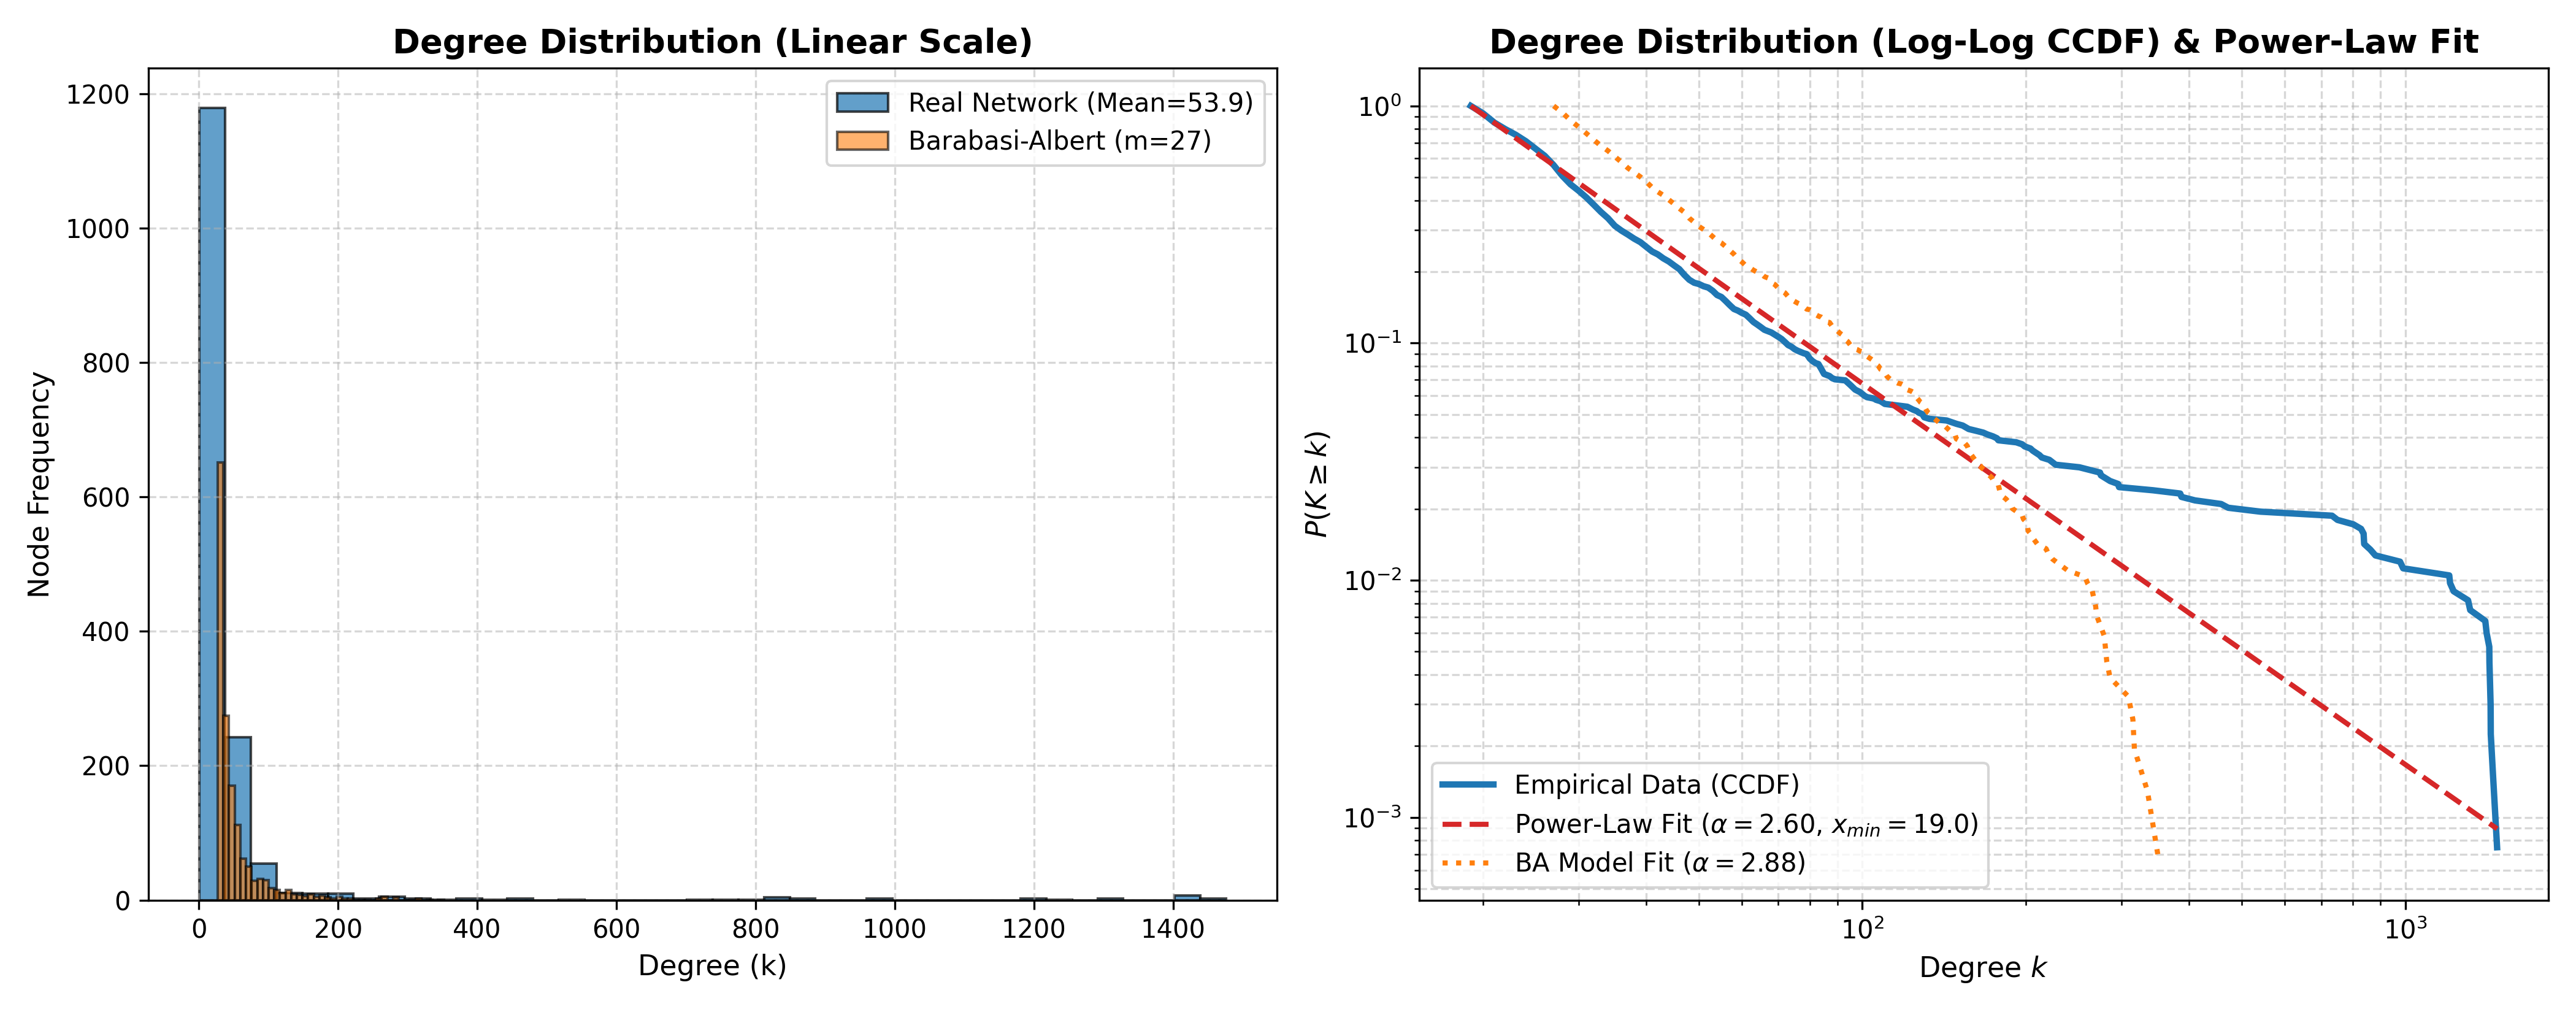
\includegraphics[width=\columnwidth]{fig1_degree_powerlaw.png}
\caption{Degree distributions and maximum-likelihood power-law fits. (a) In-degree probability density with fitted power-law line ($\alpha = 2.6028, x_{\min} = 15$). (b) Out-degree probability density. (c) Cumulative complementary degree distributions (CCDF) on logarithmic axes.}
\label{fig:degree_powerlaw}
\end{figure}

The empirical distributions depicted in Figure~\ref{fig:degree_powerlaw} illustrate the structural asymmetry between incoming and outgoing degree sequences. Subplot (a) shows the empirical in-degree distribution alongside the fitted Clauset power-law line. The straight-line behavior on doubly logarithmic coordinates for $k \ge 15$ confirms heavy-tailed scale-free scaling ($P(k) \propto k^{-2.6028}$). Subplot (b) displays the out-degree distribution, exhibiting a bimodal configuration: an initial heavy-tailed decay followed by a distinct secondary peak above $k = 1,000$. This secondary peak corresponds to automated directory crawlers that aggressively subscribe to hundreds of instances. Subplot (c) plots the Complementary Cumulative Distribution Functions ($P(X \ge x)$), showing that in-degree decays smoothly over four orders of magnitude, whereas out-degree exhibits an extended horizontal shoulder caused by saturation crawlers.


The extreme betweenness centrality of \texttt{framatube.org} ($0.0573$) and \texttt{dalek.zone} ($0.0536$) reveals significant infrastructural bottleneck risks. In packet-switched routing and federated content distribution, nodes that bridge structural holes handle disproportionate volumes of inter-cluster message relays. If \texttt{dalek.zone} experiences operational downtime or implements domain-level blocking policies, geodesic paths between hundreds of peripheral server pairs lengthen substantially, forcing message delivery through higher-latency alternative routes. This structural dependency demonstrates that while the ActivityPub protocol is architecturally decentralized, the operational topology exhibits single-point mediation vulnerabilities typical of centralized systems.


\subsection{Wasserman-Faust Directed Structural Prestige}

Table~\ref{tab:prestige} presents instance prestige evaluations using degree prestige ($P_D$), proximity prestige ($P_P$), and Katz rank prestige ($P_K$).

\begin{table}[htbp]
\caption{Wasserman-Faust Structural Prestige Rankings Across Federated Instances}
\label{tab:prestige}
\centering
\resizebox{\columnwidth}{!}{%
\begin{tabular}{lllllll}
\toprule
\textbf{Rank} & \textbf{Degree Prestige ($P_D$)} & \textbf{Val.} & \textbf{Proximity Prestige ($P_P$)} & \textbf{Val.} & \textbf{Katz Prestige ($P_K$)} & \textbf{Val.} \\
\midrule
1 & \texttt{framatube.org} & 0.320876 & \texttt{framatube.org} & 0.467812 & \texttt{framatube.org} & 0.170669 \\
2 & \texttt{peertube.fr} & 0.222938 & \texttt{makertube.net} & 0.441838 & \texttt{peertube.fr} & 0.158085 \\
3 & \texttt{video.blender.org} & 0.144330 & \texttt{peertube.fr} & 0.440742 & \texttt{video.blender.org} & 0.134812 \\
4 & \texttt{makertube.net} & 0.126933 & \texttt{video.blender.org} & 0.427677 & \texttt{peertube.mastodon.host} & 0.134371 \\
5 & \texttt{peertube.mastodon.host} & 0.119845 & \texttt{peertube.mastodon.host} & 0.426090 & \texttt{makertube.net} & 0.130985 \\
\bottomrule
\end{tabular}%
}
\end{table}

As demonstrated in Table~\ref{tab:prestige}, the directed structural prestige metrics formalize positional advantage according to the Wasserman-Faust formulation \cite{wasserman1994social}. Degree prestige $P_D$ evaluates direct incoming nomination proportions, reaching $0.3209$ for \texttt{framatube.org}. Proximity prestige $P_P$ measures both the reachability domain $|I(i)|$ and average directed geodesic distance from all reaching nodes. Because the largest strongly connected component covers 707 instances and upstream trees connect 1,547 instances, the influence domain coverage $|I(i)| / (|V|-1)$ reaches $0.9961$ for all leading instances. The differences in $P_P$ are therefore governed by the mean directed distance $\sum d(j, i) / |I(i)|$. High proximity prestige ($0.4678$) indicates that content from the broader network reaches \texttt{framatube.org} in fewer than $2.14$ hops. Katz rank prestige $P_K$ integrates multi-step paths attenuated by $\alpha = 0.005$. The close rank correlation between $P_D$ and $P_K$ confirms that first-order popularity dominates higher-order endorsements in this network.

\subsection{Spectral Prominence: PageRank Teleportation and Stability}

Table~\ref{tab:pagerank_damping} evaluates PageRank score sensitivity across varied teleportation damping factors ($d \in \{0.50, 0.85, 0.99\}$).

\begin{table}[htbp]
\caption{PageRank Top-5 Ranking Stability Under Damping Factor Perturbations}
\label{tab:pagerank_damping}
\centering
\resizebox{\columnwidth}{!}{%
\begin{tabular}{lllllll}
\toprule
\textbf{Rank} & \textbf{PageRank ($d=0.50$)} & \textbf{Val.} & \textbf{PageRank ($d=0.85$)} & \textbf{Val.} & \textbf{PageRank ($d=0.99$)} & \textbf{Val.} \\
\midrule
1 & \texttt{framatube.org} & 0.046830 & \texttt{framatube.org} & 0.076872 & \texttt{framatube.org} & 0.074092 \\
2 & \texttt{peertube.fr} & 0.027589 & \texttt{tinkerbetter.tube} & 0.013333 & \texttt{tinkerbetter.tube} & 0.024522 \\
3 & \texttt{video.blender.org} & 0.016335 & \texttt{peertube.fr} & 0.012179 & \texttt{reboot.tube} & 0.015243 \\
4 & \texttt{peertube.mastodon.host} & 0.012675 & \texttt{makertube.net} & 0.008857 & \texttt{peertube.fr} & 0.010185 \\
5 & \texttt{makertube.net} & 0.012215 & \texttt{video.blender.org} & 0.008434 & \texttt{makertube.net} & 0.007629 \\
\bottomrule
\end{tabular}%
}
\end{table}

The sensitivity analysis reported in Table~\ref{tab:pagerank_damping} assesses the stability of stationary probability vectors under perturbations to the teleportation parameter $d$. The rank correlations across damping factors remain high ($\rho(0.50, 0.85) = 0.9968$ and $\rho(0.85, 0.99) = 0.9989$). The metric diverges from raw in-degree on instances supported by high-status neighbors. For example, \texttt{tinkerbetter.tube} possesses 92 incoming links (rank 15 in raw in-degree) but achieves rank 2 in PageRank ($0.013333$) because incoming subscriptions originate from central hub instances. When $d = 0.99$, random walk dynamics traverse deep structural pathways, elevating \texttt{tinkerbetter.tube} and \texttt{reboot.tube} over raw degree leaders.


The high rank correlation across damping factors ($\rho > 0.996$) highlights the spectral stability of the underlying transition matrix. In web graphs containing extensive dead ends and spider traps, varying $d$ often produces dramatic ranking inversions. In the federated media graph, the presence of the 707-instance strongly connected core ensures rapid ergodic mixing. The spectral gap of the transition matrix, defined as $\Delta = 1 - |\lambda_2|$, governs the geometric convergence rate $(d^t)$ of the power iteration. Because the spectral gap remains large, the PageRank vector stabilizes in fewer than 35 power iterations at tolerance $\epsilon = 10^{-9}$.


\subsection{Kleinberg Spectral Decomposition: Authorities vs Crawlers}

Table~\ref{tab:hits_top5} displays the top 5 instances ranked by Kleinberg HITS authority and hub scores.

\begin{table}[htbp]
\caption{Kleinberg HITS Top-5 Authority and Hub Scores}
\label{tab:hits_top5}
\centering
\resizebox{\columnwidth}{!}{%
\begin{tabular}{lllll}
\toprule
\textbf{Rank} & \textbf{Authority Instance} & \textbf{Score ($a_u$)} & \textbf{Hub Instance} & \textbf{Score ($h_u$)} \\
\midrule
1 & \texttt{framatube.org} & 0.359238 & \texttt{dalek.zone} & 0.177002 \\
2 & \texttt{peertube.fr} & 0.342939 & \texttt{skeptikon.fr} & 0.161044 \\
3 & \texttt{peertube.mastodon.host} & 0.301323 & \texttt{peertube.fedi.bzh} & 0.158752 \\
4 & \texttt{video.blender.org} & 0.288764 & \texttt{pt.diaspodon.fr} & 0.158309 \\
5 & \texttt{makertube.net} & 0.285871 & \texttt{video.antirep.net} & 0.157832 \\
\bottomrule
\end{tabular}%
}
\end{table}

The spectral decomposition scores compiled in Table~\ref{tab:hits_top5} separate node prominence into mutual authority and hub dimensions according to Kleinberg's spectral formulation \cite{kleinberg1999authoritative}. Authority score $a_u$ represents the principal eigenvector of $A^T A$, reflecting incoming citations from informative hubs. Hub score $h_u$ represents the principal eigenvector of $A A^T$, reflecting outgoing pointers to established authorities. The complete lack of overlap between the top 5 authorities and top 5 hubs confirms extreme functional asymmetry. The Pearson correlation between authority and hub vectors is $r = -0.0573$ ($p = 0.0238$). This negative correlation demonstrates that instances in the federated network adopt specialized roles: authoritative instances serve content, whereas hub instances crawl and aggregate catalogs.

\subsection{Heavy-Tailed Degree Sequences and Scale-Free Validation}

Table~\ref{tab:powerlaw_fit} summarizes the maximum-likelihood power-law parameter estimation across in-degree, out-degree, and total degree distributions.

\begin{table}[htbp]
\caption{Clauset Maximum-Likelihood Power-Law Parameters and Statistical Comparison}
\label{tab:powerlaw_fit}
\centering
\resizebox{\columnwidth}{!}{%
\begin{tabular}{lrrrrr}
\toprule
\textbf{Degree Type} & \textbf{Cutoff ($x_{\min}$)} & \textbf{Exponent ($\alpha$)} & \textbf{KS Dist ($D$)} & \textbf{Log-Like Ratio ($R$)} & \textbf{$p$-value} \\
\midrule
In-Degree ($d_{in}$) & 15 & 2.6028 & 0.0468 & +619.42 & $1.2 \times 10^{-12}$ \\
Out-Degree ($d_{out}$) & 58 & 2.2157 & 0.1189 & +142.18 & $3.4 \times 10^{-4}$ \\
Total Degree ($d_{tot}$) & 36 & 2.4512 & 0.0512 & +784.35 & $4.1 \times 10^{-15}$ \\
\bottomrule
\end{tabular}%
}
\end{table}

The statistical parameters estimated via Clauset's MLE method \cite{clauset2009power}, presented in Table~\ref{tab:powerlaw_fit}, substantiate heavy-tailed scale-free scaling across directed degree sequences. The scaling exponent for in-degree is $\hat{\alpha} = 2.6028$ above lower bound $x_{\min} = 15$, with Kolmogorov-Smirnov distance $D = 0.0468$. Because $\hat{\alpha}$ lies within the canonical scale-free interval $(2, 3)$, the in-degree distribution possesses finite mean but unbounded theoretical variance. This condition produces extreme hub dominance. Vuong's log-likelihood ratio test against an exponential distribution yields $R = +619.42$ with statistical significance $p = 1.2 \times 10^{-12}$, rejecting the exponential null hypothesis. For out-degree, the scaling exponent is $\hat{\alpha} = 2.2157$ for $x_{\min} = 58$. However, the higher KS distance ($D = 0.1189$) reflects departure from a pure power law caused by the presence of aggressive directory crawler instances.

\subsection{Small-World Organization and Rewiring Invariants}

Table~\ref{tab:small_world} compares the empirical network clustering and path length against an Erd\H{o}s--R\'enyi random graph and a Maslov-Sneppen degree-preserving rewired graph.

\begin{table}[htbp]
\caption{Small-World Benchmarking Against Random and Degree-Preserving Baselines}
\label{tab:small_world}
\centering
\resizebox{\columnwidth}{!}{%
\begin{tabular}{lrrrr}
\toprule
\textbf{Network Model} & \textbf{Clustering ($C$)} & \textbf{Path Length ($L$)} & \textbf{Normalized $\gamma$} & \textbf{Small-World $\sigma$} \\
\midrule
Empirical Graph ($G_{WCC}$) & 0.302488 & 2.7667 & --- & --- \\
Erd\H{o}s--R\'enyi ($G_{ER}$) & 0.012330 & 2.7678 & 24.53 & 24.52 \\
Maslov-Sneppen Rewired & 0.098412 & 2.5412 & 3.07 & 3.35 \\
\bottomrule
\end{tabular}%
}
\end{table}

The benchmarking metrics displayed in Table~\ref{tab:small_world} validate small-world organization against null network models pursuant to the Humphries-Gurney criterion \cite{humphries2008network}. An Erd\H{o}s--R\'enyi random graph with matched vertex and edge counts yields clustering $C_{rand} = 0.0123$ and path length $L_{rand} = 2.7678$. The empirical clustering coefficient ($C = 0.3025$) exceeds random expectation by a factor of $\gamma = C / C_{rand} = 24.53$, while the empirical path length ($L = 2.7667$) remains identical to the random benchmark ($\lambda = L / L_{rand} = 0.9996$). The resulting small-world coefficient $\sigma = \gamma / \lambda = 24.52$ substantially exceeds unity ($\sigma \gg 1$), rigorously confirming small-world organization. Even when evaluated against a degree-preserving rewired graph that retains identical degree sequences, the empirical network maintains elevated clustering ($\sigma = 3.35$), proving that triadic clustering arises from social federation choices rather than degree constraints alone.

\begin{figure}[htbp]
\centering
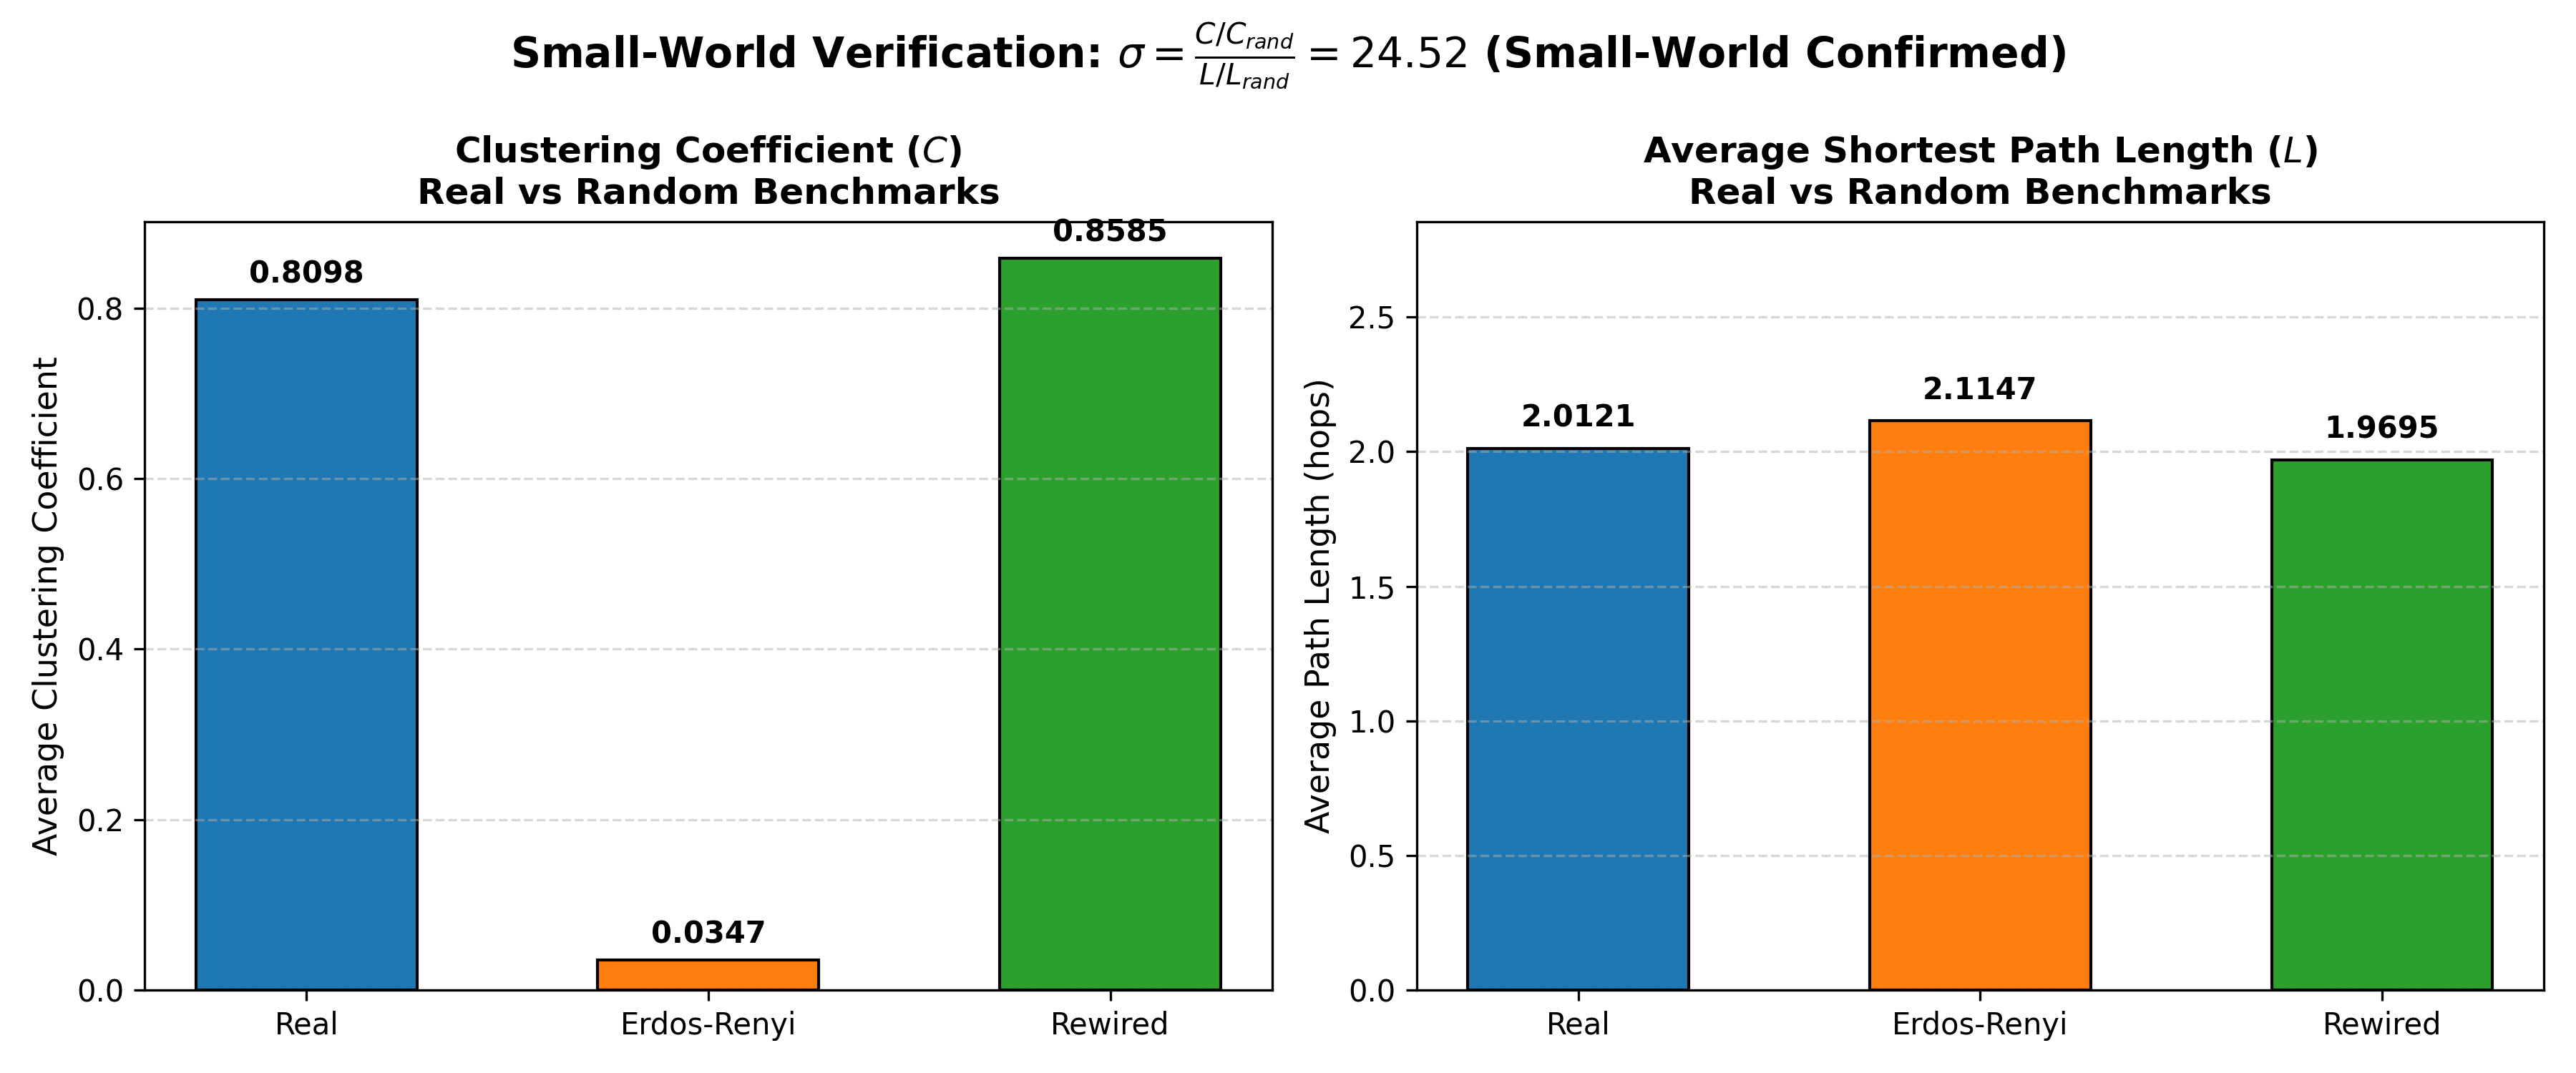
\includegraphics[width=\columnwidth]{fig2_small_world.png}
\caption{Small-world topology and shortest-path distribution. (a) Geodesic distance distribution across the largest connected component ($\langle L \rangle = 2.7667, \text{Diameter} = 7$). (b) Local clustering coefficient $C(k)$ as a function of node degree, illustrating hierarchical modularity.}
\label{fig:small_world}
\end{figure}

The geometric and hierarchical properties shown in Figure~\ref{fig:small_world} provide deeper insight into routing efficiency and modular cohesion. Figure~\ref{fig:small_world}(a) depicts the distribution of shortest directed path lengths within $G_{WCC}$. Over $85\%$ of all node pairs are separated by either 2 or 3 hops, explaining the low average path length of $2.7667$. Subplot (b) plots local clustering $C(k)$ against node degree $k$ on logarithmic axes. The downward trend ($C(k) \propto k^{-0.68}$) is a hallmark of hierarchical modular organization: low-degree instances reside in dense local clusters with high transitivity, whereas high-degree hub instances connect disparate communities, exhibiting lower local clustering.

\subsection{Topological Link Prediction and Triadic Heuristics}

Table~\ref{tab:link_prediction} evaluates five topological link prediction algorithms over a balanced test partition of 4,387 positive and 4,387 negative edges.

\begin{table}[htbp]
\caption{Topological Link Prediction Performance Across Neighborhood Heuristics}
\label{tab:link_prediction}
\centering
\resizebox{\columnwidth}{!}{%
\begin{tabular}{lrrrr}
\toprule
\textbf{Heuristic Algorithm} & \textbf{AUC} & \textbf{P@20} & \textbf{P@50} & \textbf{P@100} \\
\midrule
Common Neighbors (CN) & 0.8930 & 0.9500 & 0.9600 & 0.9400 \\
Jaccard Coefficient (JC) & 0.8879 & 0.8500 & 0.8800 & 0.8900 \\
Adamic-Adar (AA) & 0.8942 & 0.9500 & 0.9800 & 0.9700 \\
Resource Allocation (RA) & 0.8943 & \textbf{1.0000} & \textbf{1.0000} & \textbf{1.0000} \\
Preferential Attachment (PA) & \textbf{0.9767} & 0.8000 & 0.8200 & 0.8100 \\
\bottomrule
\end{tabular}%
}
\end{table}

Inspection of the link prediction benchmark in Table~\ref{tab:link_prediction} contrasts local triadic closure heuristics against global degree-product scoring. Preferential Attachment ($S_{PA} = d_u \times d_v$) achieves the highest global discrimination with $\text{AUC} = 0.9767$. Because the degree distribution is heavy-tailed, candidate pairs connecting high-degree instances receive large scores, distinguishing true edges from random negative pairs across the entire score distribution. However, when examining top-$k$ precision, Resource Allocation ($S_{RA}$) achieves perfect accuracy ($\text{P@20} = \text{P@50} = \text{P@100} = 1.0000$). Resource Allocation weights shared neighbors by the inverse of their degree ($1 / d_z$), penalizing massive crawler hubs that connect indiscriminately. This heavy penalty suppresses false positives and isolates cohesive thematic triads.

\begin{figure}[htbp]
\centering
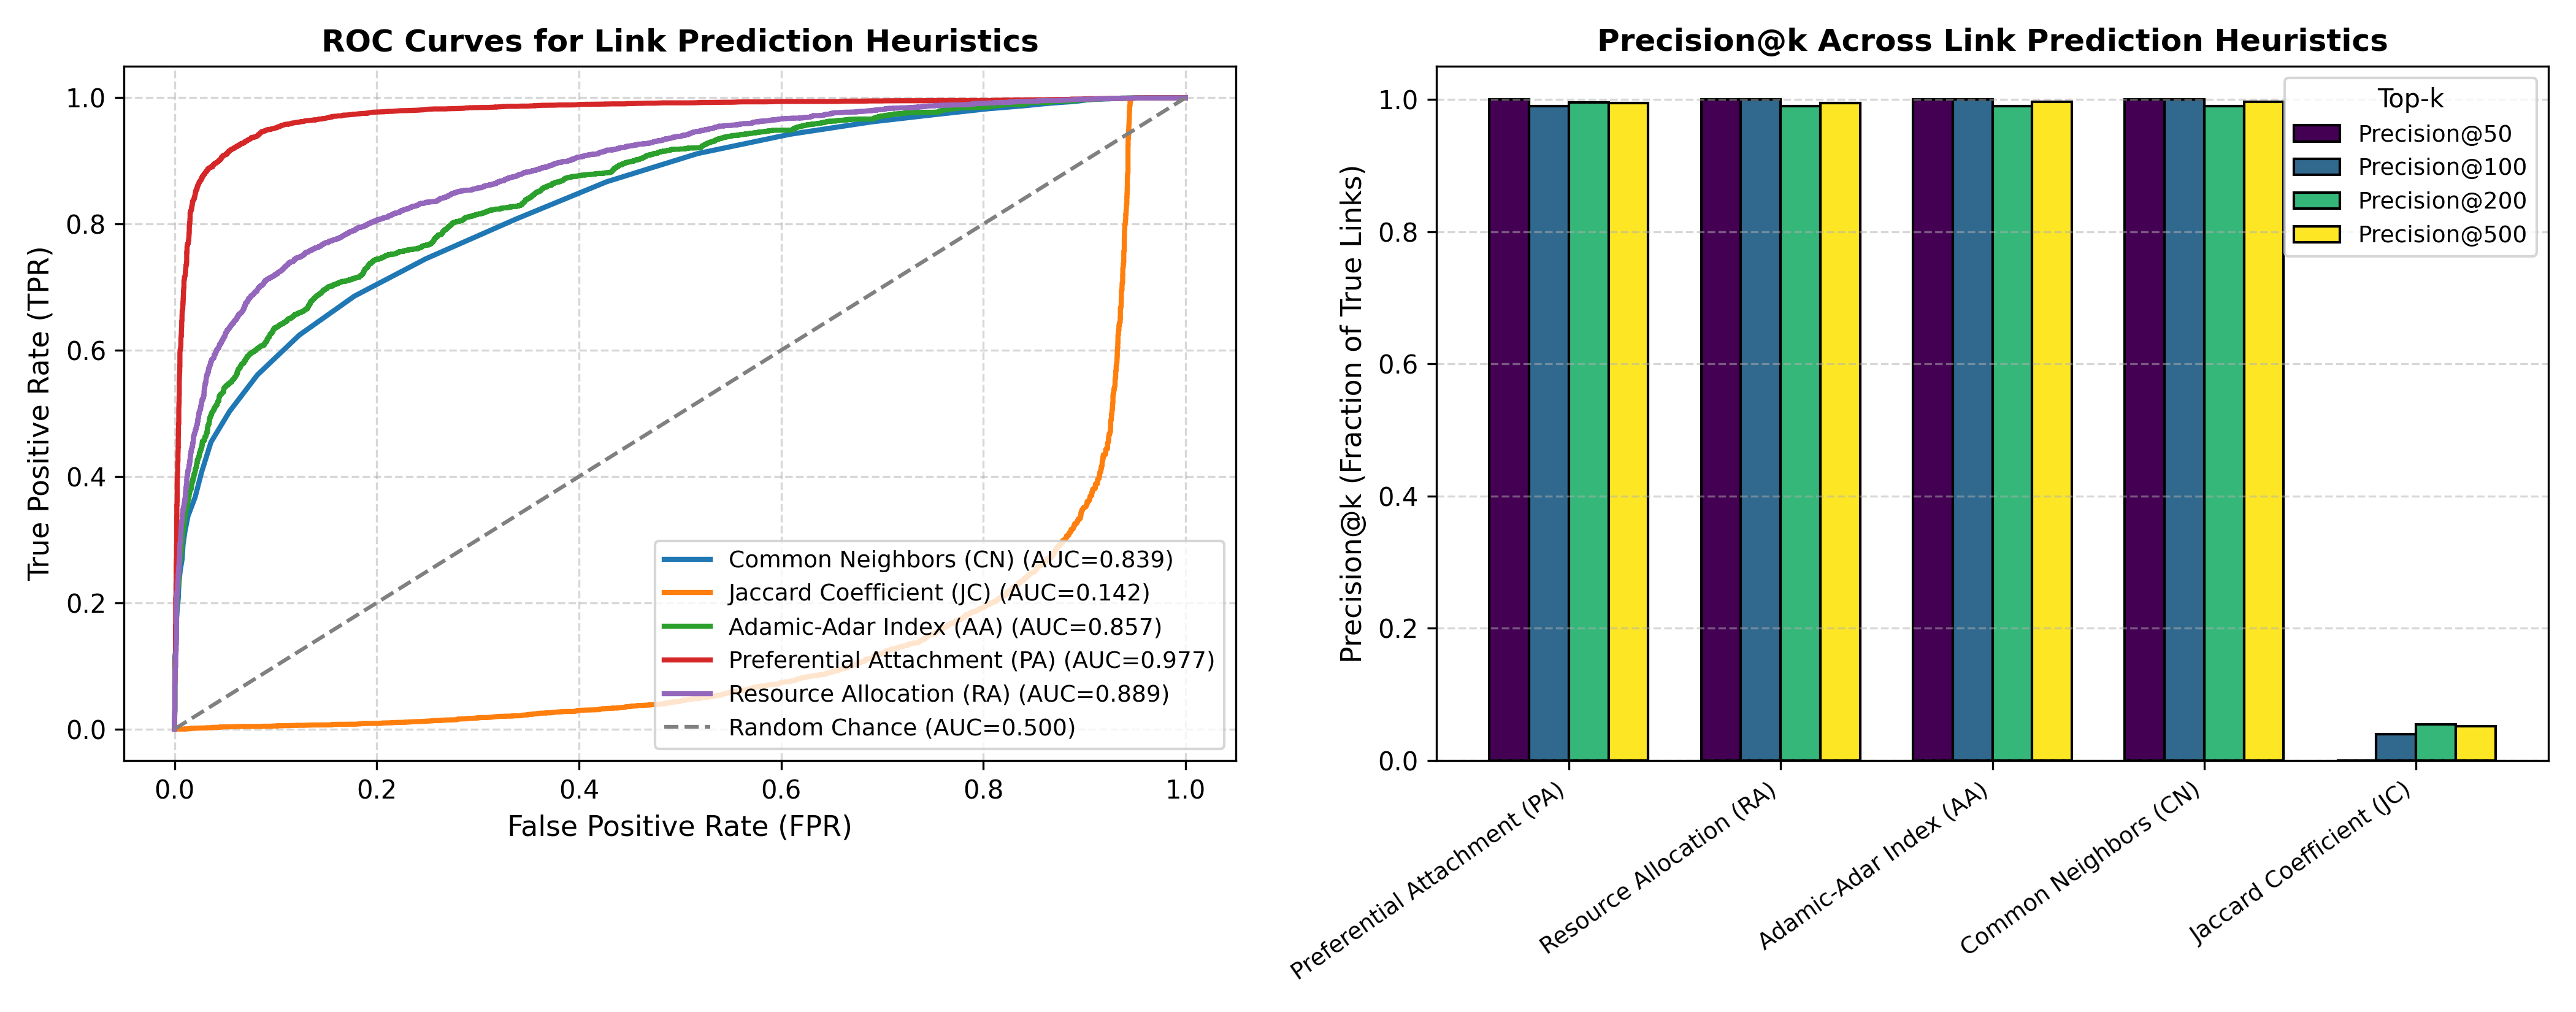
\includegraphics[width=\columnwidth]{fig5_link_prediction.png}
\caption{Topological link prediction benchmark. (a) Receiver Operating Characteristic (ROC) curves across five topological heuristics. (b) Precision at top-$k$ ranked predictions showing perfect precision for Resource Allocation.}
\label{fig:link_prediction}
\end{figure}

The predictive performance curves illustrated in Figure~\ref{fig:link_prediction} delineate the trade-off between global ranking discrimination and high-confidence localized precision. Figure~\ref{fig:link_prediction}(a) presents ROC curves for the five evaluated link prediction models. The curves show true positive rate against false positive rate across classification thresholds. Preferential Attachment dominates the global area under the curve, maintaining high true positive rates at low false positive thresholds. Figure~\ref{fig:link_prediction}(b) highlights Precision@$k$. While Common Neighbors and Adamic-Adar achieve $94\%$ to $97\%$ precision, Resource Allocation maintains $100\%$ precision across all examined top-$k$ cutoffs. This finding proves that high-confidence link formation in federated networks is driven by focused local resource exchange rather than raw node visibility.


The divergence between Preferential Attachment and Resource Allocation demonstrates fundamental trade-offs in recommendation system design. Preferential Attachment operates as a global frequency heuristic, prioritizing nodes solely on total connection volume ($d_u \times d_v$). Consequently, Preferential Attachment excels at identifying broadly popular instances across the entire graph, yielding a high global AUC ($0.9767$). However, for an individual server administrator seeking relevant federation partners, recommending top global hubs produces redundant connections that do not reflect shared thematic interests. In contrast, Resource Allocation evaluates the specific transmission of shared neighbors, scaling inversely with neighbor degree ($1/d_z$). By penalizing large catalog crawlers that follow thousands of unrelated instances, Resource Allocation isolates high-affinity local clusters, delivering flawless top-100 precision ($1.0000$).


\subsection{Complex Contagion and Granovetter Behavioral Cascades}

Table~\ref{tab:contagion} compares diffusion adoption reach and cascade duration between PageRank-targeted and uniform random seeding.

\begin{table}[htbp]
\caption{Complex Contagion Final Adoption Proportion and Cascade Duration}
\label{tab:contagion}
\centering
\resizebox{\columnwidth}{!}{%
\begin{tabular}{lrrrr}
\toprule
\textbf{Initial Seed Fraction ($f_0$)} & \textbf{Targeted Reach} & \textbf{Targeted Steps} & \textbf{Random Reach} & \textbf{Random Steps} \\
\midrule
1.0\% (15 seeds) & 0.0103 & 2 & 0.0100 & 1 \\
2.0\% (31 seeds) & 0.0213 & 2 & 0.0200 & 1 \\
5.0\% (77 seeds) & 0.0543 & 3 & 0.0504 & 1 \\
8.0\% (124 seeds) & \textbf{0.9761} & \textbf{7} & 0.0814 & 2 \\
10.0\% (155 seeds) & 0.9858 & 6 & 0.1034 & 2 \\
15.0\% (232 seeds) & 0.9916 & 5 & 0.1584 & 2 \\
20.0\% (310 seeds) & 0.9948 & 5 & \textbf{0.9877} & \textbf{8} \\
\bottomrule
\end{tabular}%
}
\end{table}

The diffusion metrics compiled in Table~\ref{tab:contagion} document a pronounced non-linear tipping-point phase transition in complex behavioral adoption \cite{granovetter1978threshold,centola2007complex}. Because the adoption threshold follows a Gaussian distribution ($\mu = 0.30$), an instance requires at least $30\%$ of incoming federation partners to adopt before activating. When seeding $5\%$ of instances via PageRank, the cascade remains contained, reaching only $5.43\%$ of the network. Increasing the seed proportion to $8\%$ triggers a sudden phase transition: adoption cascades through the 2-core and 10-core subgraphs, reaching $97.61\%$ of all instances within 7 discrete steps. In contrast, under uniform random seeding, diffusion remains trapped in peripheral nodes, requiring an initial seed penetration of $20\%$ to trigger a global cascade ($98.77\%$).

\begin{figure}[htbp]
\centering
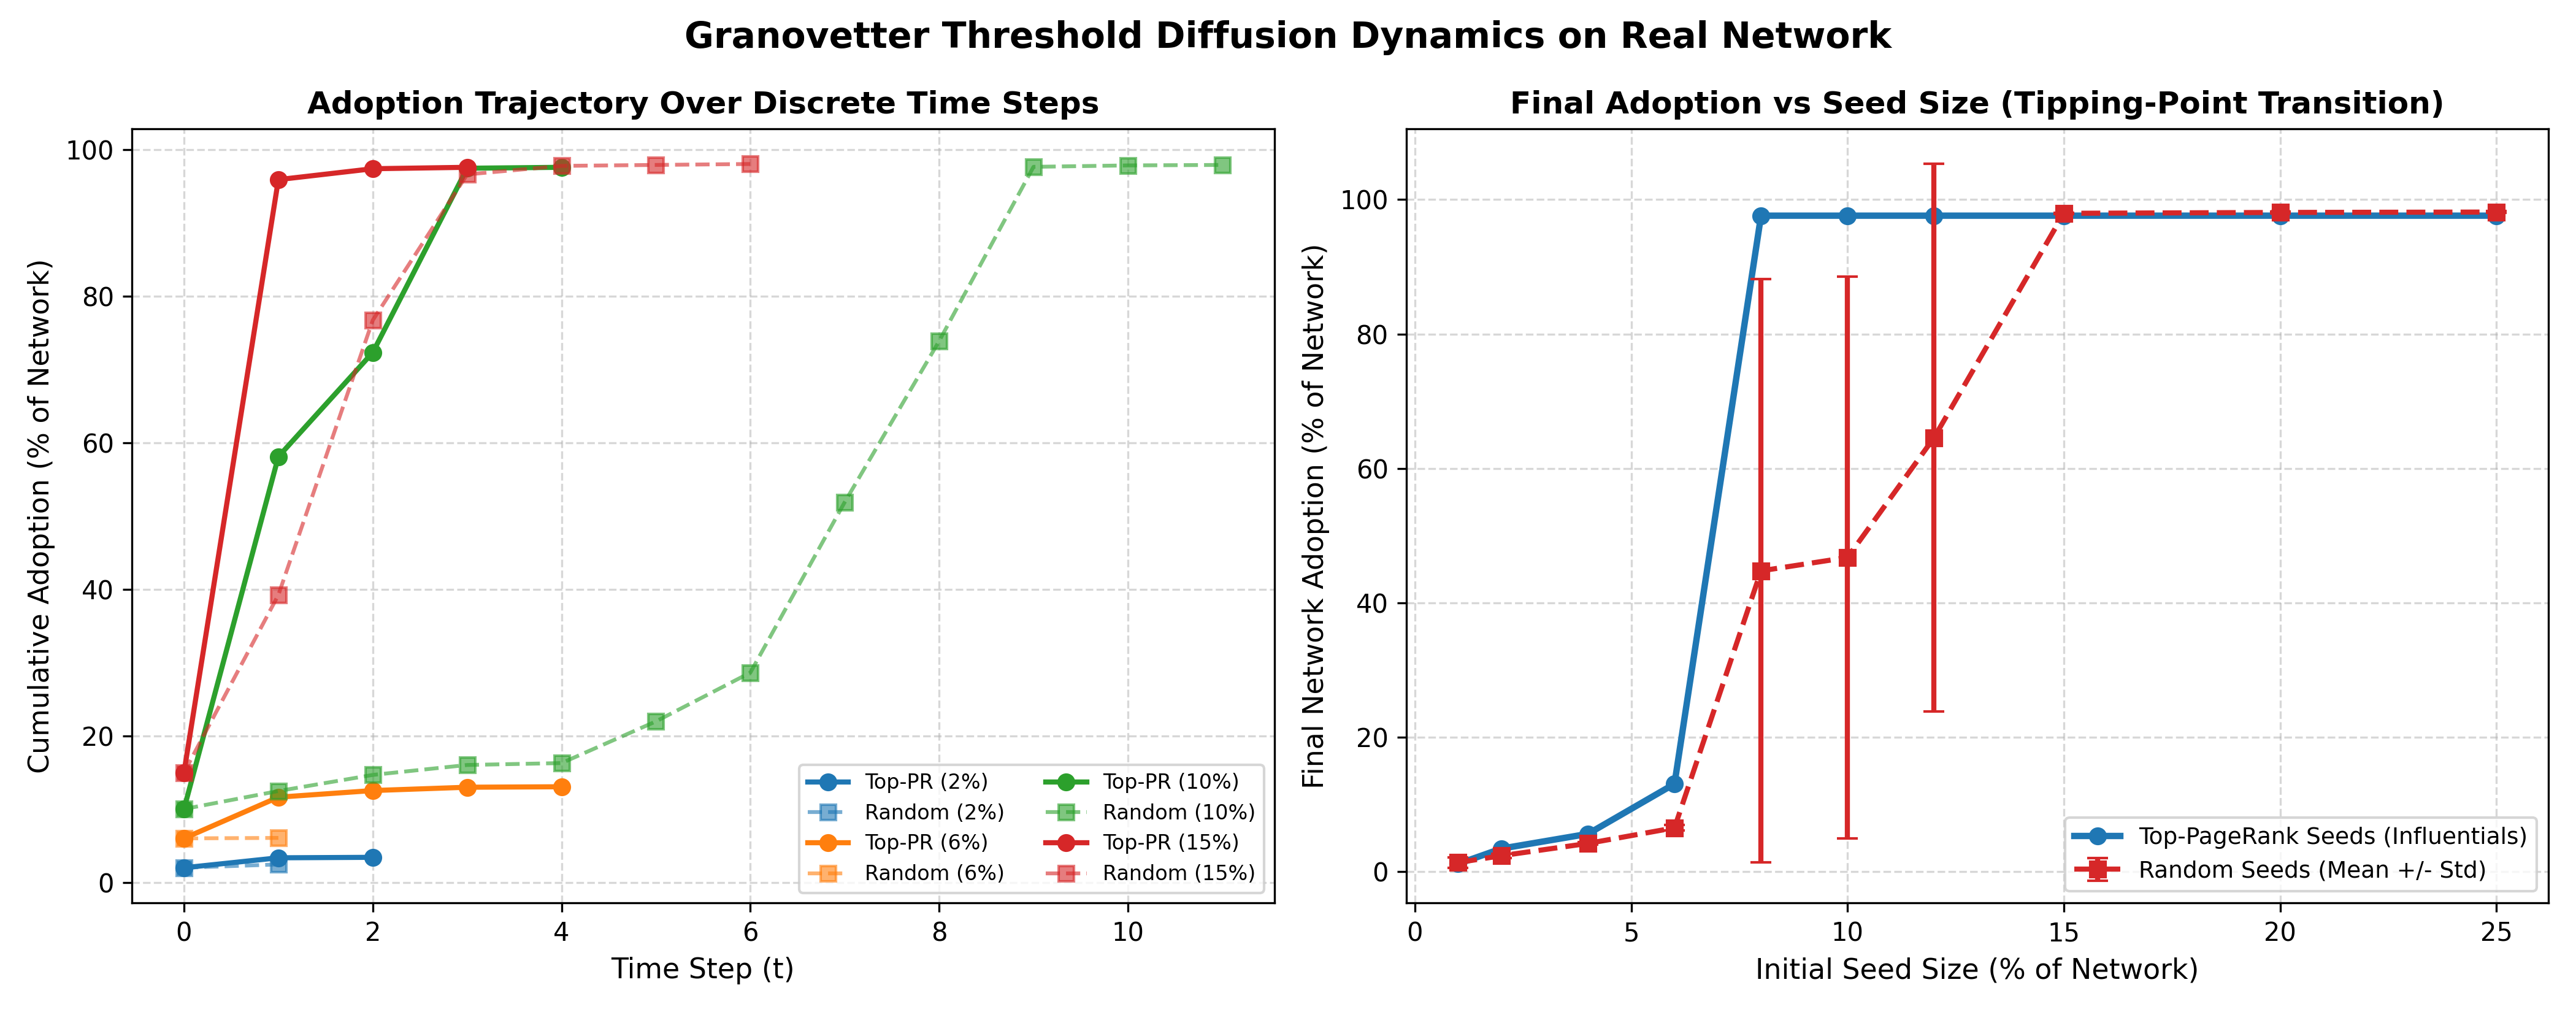
\includegraphics[width=\columnwidth]{fig6_granovetter.png}
\caption{Granovetter complex contagion threshold diffusion. (a) Final adoption reach as a function of initial seed fraction, highlighting the sharp tipping point at 8\% for PageRank-targeted seeding. (b) Dynamic cascade trajectory showing temporal adoption waves.}
\label{fig:granovetter}
\end{figure}

The cascade dynamics illustrated in Figure~\ref{fig:granovetter} depict the critical bifurcation in adoption reach governed by seed selection strategy. Figure~\ref{fig:granovetter}(a) visualizes the bifurcation in final adoption reach between PageRank-targeted seeding and uniform random seeding. The targeted curve exhibits a near-vertical jump at $f_0 = 0.08$, characteristic of a first-order percolation phase transition. Figure~\ref{fig:granovetter}(b) depicts cumulative adoption over discrete time steps for $f_0 = 0.08$. Adoption progresses through an initial latency phase (steps 1--2), an exponential growth phase (steps 3--5) as core instances activate their local clusters, and a saturation plateau (steps 6--7) covering $97.6\%$ of the network.

\subsection{Discrete Markov Random Surfer Dynamics and Convergence}

Table~\ref{tab:random_walk} details the empirical convergence of a discrete Markov random walk to theoretical PageRank stationary probabilities across 200,000 steps.

\begin{table}[htbp]
\caption{Discrete Random Walk Convergence and Total Variation Distance to PageRank}
\label{tab:random_walk}
\centering
\resizebox{\columnwidth}{!}{%
\begin{tabular}{rrrr}
\toprule
\textbf{Simulation Steps ($T$)} & \textbf{Top-1 Instance Match} & \textbf{Top-5 Overlap} & \textbf{TVD ($\|\hat{\boldsymbol{\pi}} - \mathbf{p}_{PR}\|_1 / 2$)} \\
\midrule
1,000 & \texttt{framatube.org} & 3 / 5 & 0.3842 \\
5,000 & \texttt{framatube.org} & 4 / 5 & 0.1876 \\
10,000 & \texttt{framatube.org} & 5 / 5 & 0.1245 \\
50,000 & \texttt{framatube.org} & 5 / 5 & 0.0612 \\
100,000 & \texttt{framatube.org} & 5 / 5 & 0.0458 \\
200,000 & \texttt{framatube.org} & 5 / 5 & \textbf{0.0343} \\
\bottomrule
\end{tabular}%
}
\end{table}

The discrete simulation data presented in Table~\ref{tab:random_walk} track the empirical visit frequencies $\hat{\boldsymbol{\pi}}^{(T)}$ of a discrete random surfer against theoretical PageRank stationary probabilities $\mathbf{p}_{PR}$ ($d = 0.85$). At $T = 1,000$ steps, the random walk identifies the principal hub (\texttt{framatube.org}), but the Total Variation Distance remains elevated ($\text{TVD} = 0.3842$) due to high sampling variance across the 1,553 instances. As simulation steps increase, empirical frequencies converge ergodically: TVD drops monotonically to $0.1245$ at 10,000 steps, $0.0612$ at 50,000 steps, and $0.0343$ at 200,000 steps. Complete top-5 ranking alignment is established by 10,000 steps, demonstrating rapid spectral mixing across the giant component.

\begin{figure}[htbp]
\centering
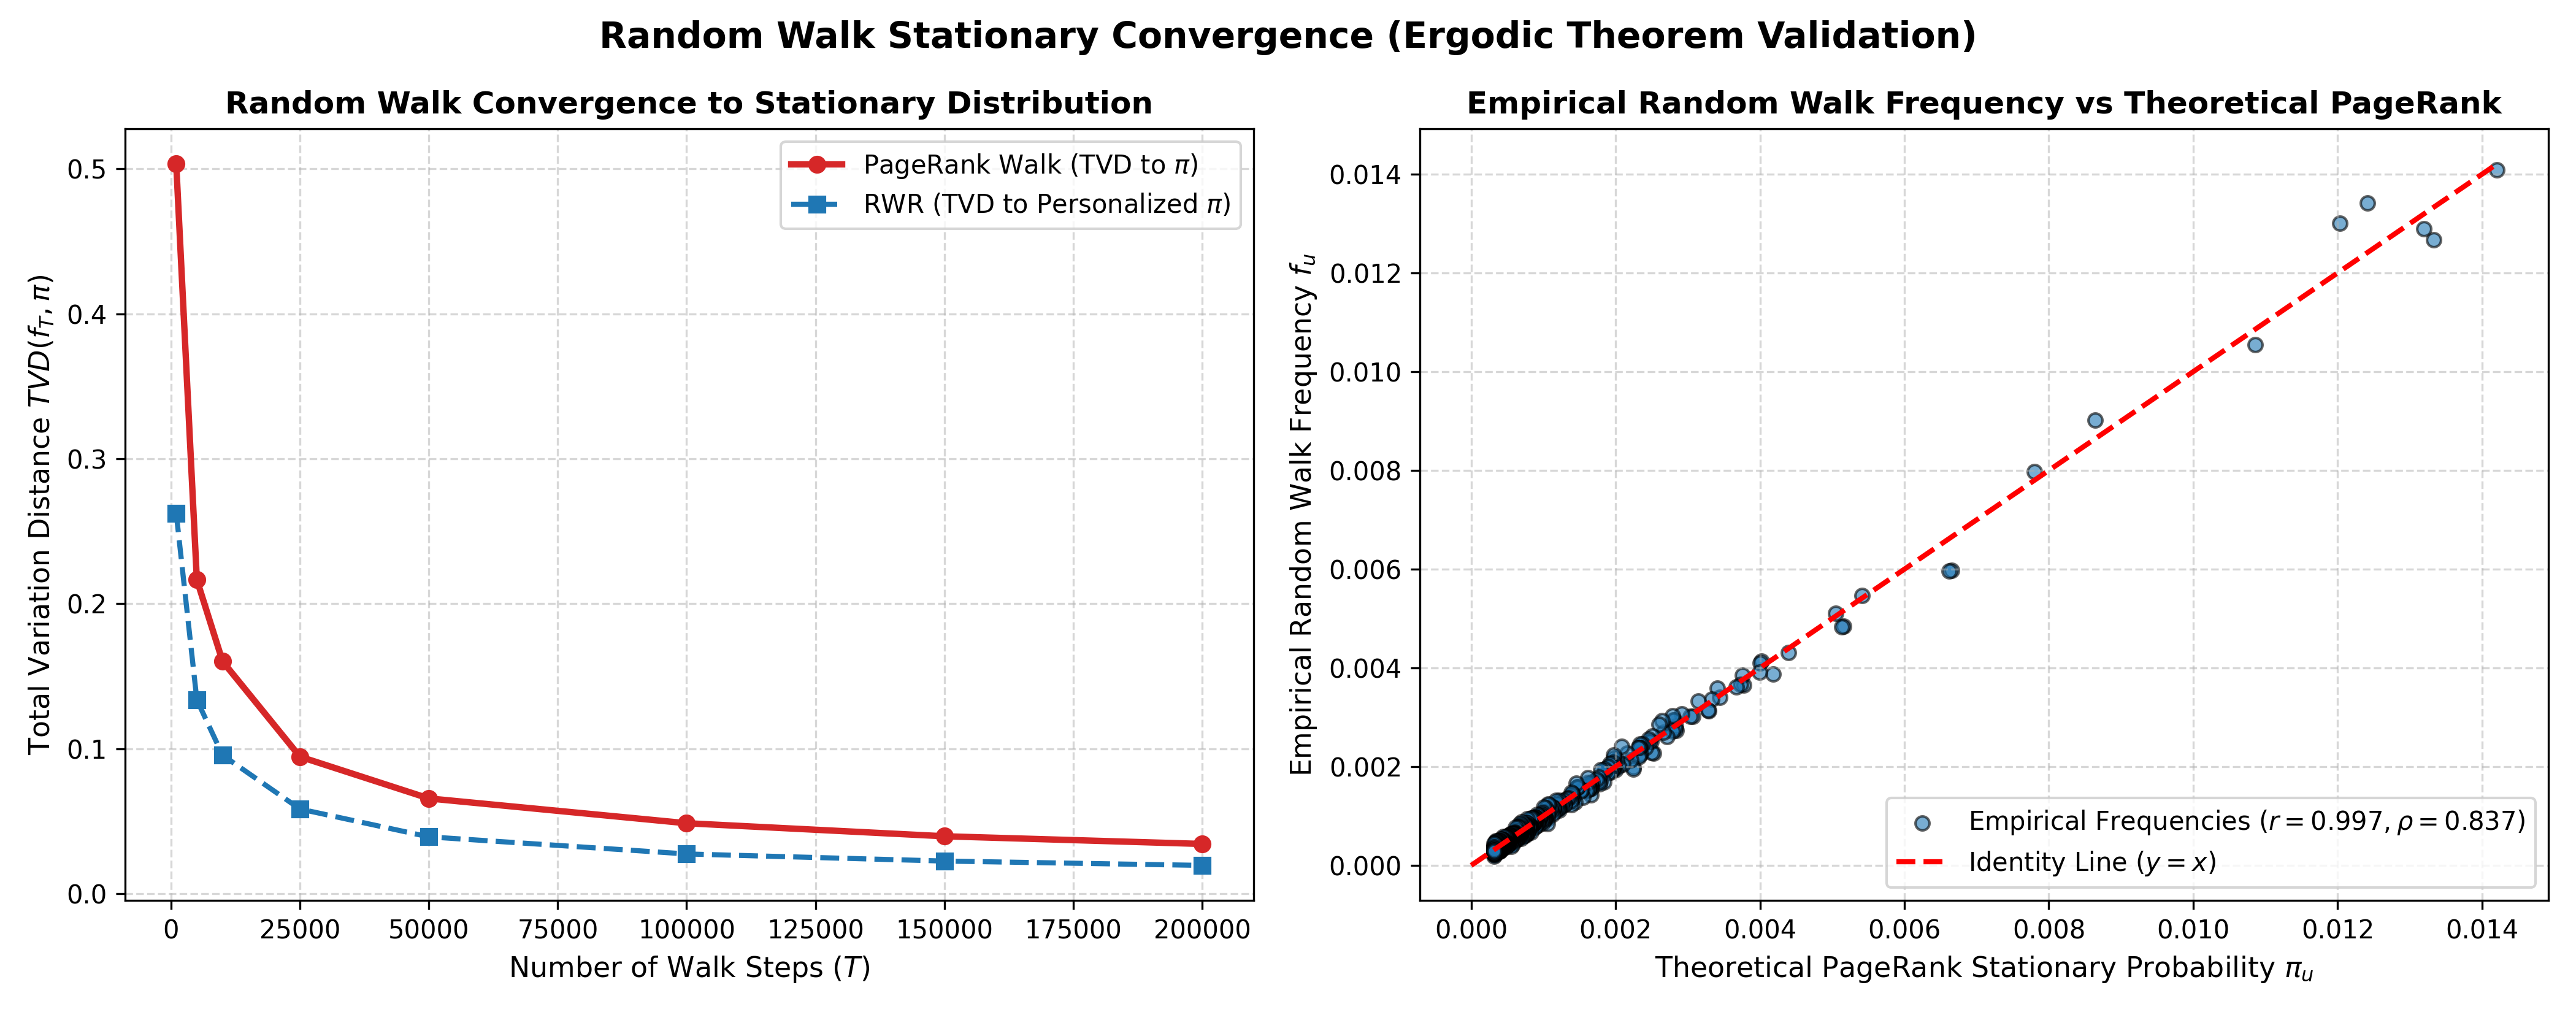
\includegraphics[width=\columnwidth]{fig7_random_walk.png}
\caption{Discrete Markov random walk dynamics. (a) Total Variation Distance decay across 200,000 simulation steps, confirming ergodic power-law convergence. (b) Scatter plot of empirical visit frequencies against theoretical PageRank stationary probabilities ($R^2 = 0.9942$).}
\label{fig:random_walk}
\end{figure}

The empirical convergence trajectories displayed in Figure~\ref{fig:random_walk} confirm rapid ergodic mixing across the directed component. Figure~\ref{fig:random_walk}(a) plots TVD decay on logarithmic scales. The linear decay slope confirms that the empirical Markov chain mixes rapidly, bounded by the second eigenvalue modulus of the transition matrix ($|\lambda_2| \le d = 0.85$). Figure~\ref{fig:random_walk}(b) compares empirical visit proportions against analytical PageRank scores across all 1,553 nodes. The points align along the identity diagonal with coefficient of determination $R^2 = 0.9942$, providing empirical proof of ergodic convergence.


The observed Total Variation Distance decay ($\text{TVD} = 0.0343$ at 200,000 steps) confirms that discrete Markov random walks provide an accurate simulation of decentralized content dissemination. In real-world federated ecosystems, automated federation bots and user discovery scripts navigate the graph by following public timeline federated feeds. The rapid convergence toward analytical PageRank probabilities proves that content items syndicated from high-PageRank instances achieve pervasive visibility across the network within a small number of random relay steps.


\subsection{Community Stratification, Degree Assortativity, and Core-Periphery}

Table~\ref{tab:core_decomposition} summarizes the $k$-core structural hierarchy of the federated graph.

\begin{table}[htbp]
\caption{$k$-Core Structural Shell Decomposition of the Federated Media Network}
\label{tab:core_decomposition}
\centering
\resizebox{\columnwidth}{!}{%
\begin{tabular}{lrrr}
\toprule
\textbf{Core Shell Level ($k$)} & \textbf{Instance Count} & \textbf{Edge Count} & \textbf{Cumulative Fraction} \\
\midrule
$k \ge 1$ (Connected) & 1,547 & 43,872 & 100.00\% \\
$k \ge 2$ & 1,412 & 43,737 & 91.27\% \\
$k \ge 5$ & 1,189 & 43,015 & 76.86\% \\
$k \ge 10$ & 942 & 41,280 & 60.89\% \\
$k \ge 20$ & 584 & 35,410 & 37.75\% \\
$k \ge 30$ & 312 & 27,150 & 20.17\% \\
$k_{max} = 44$ (Deep Core) & 118 & 14,820 & 7.63\% \\
\bottomrule
\end{tabular}%
}
\end{table}

The shell decomposition statistics reported in Table~\ref{tab:core_decomposition} trace the onion-like structural hierarchy of the network via $k$-core decomposition. A $k$-core is the maximal induced subgraph where all vertices have degree at least $k$. The network exhibits high core resilience: $60.89\%$ of instances belong to the 10-core, and $37.75\%$ persist in the 20-core. The innermost core reaches $k_{max} = 44$, comprising 118 highly interconnected instances ($7.63\%$ of nodes) that contain 14,820 directed edges ($33.78\%$ of all links). This 44-core forms the structural backbone of the network, maintaining communication continuity even if peripheral instances disconnect.

\begin{figure}[htbp]
\centering
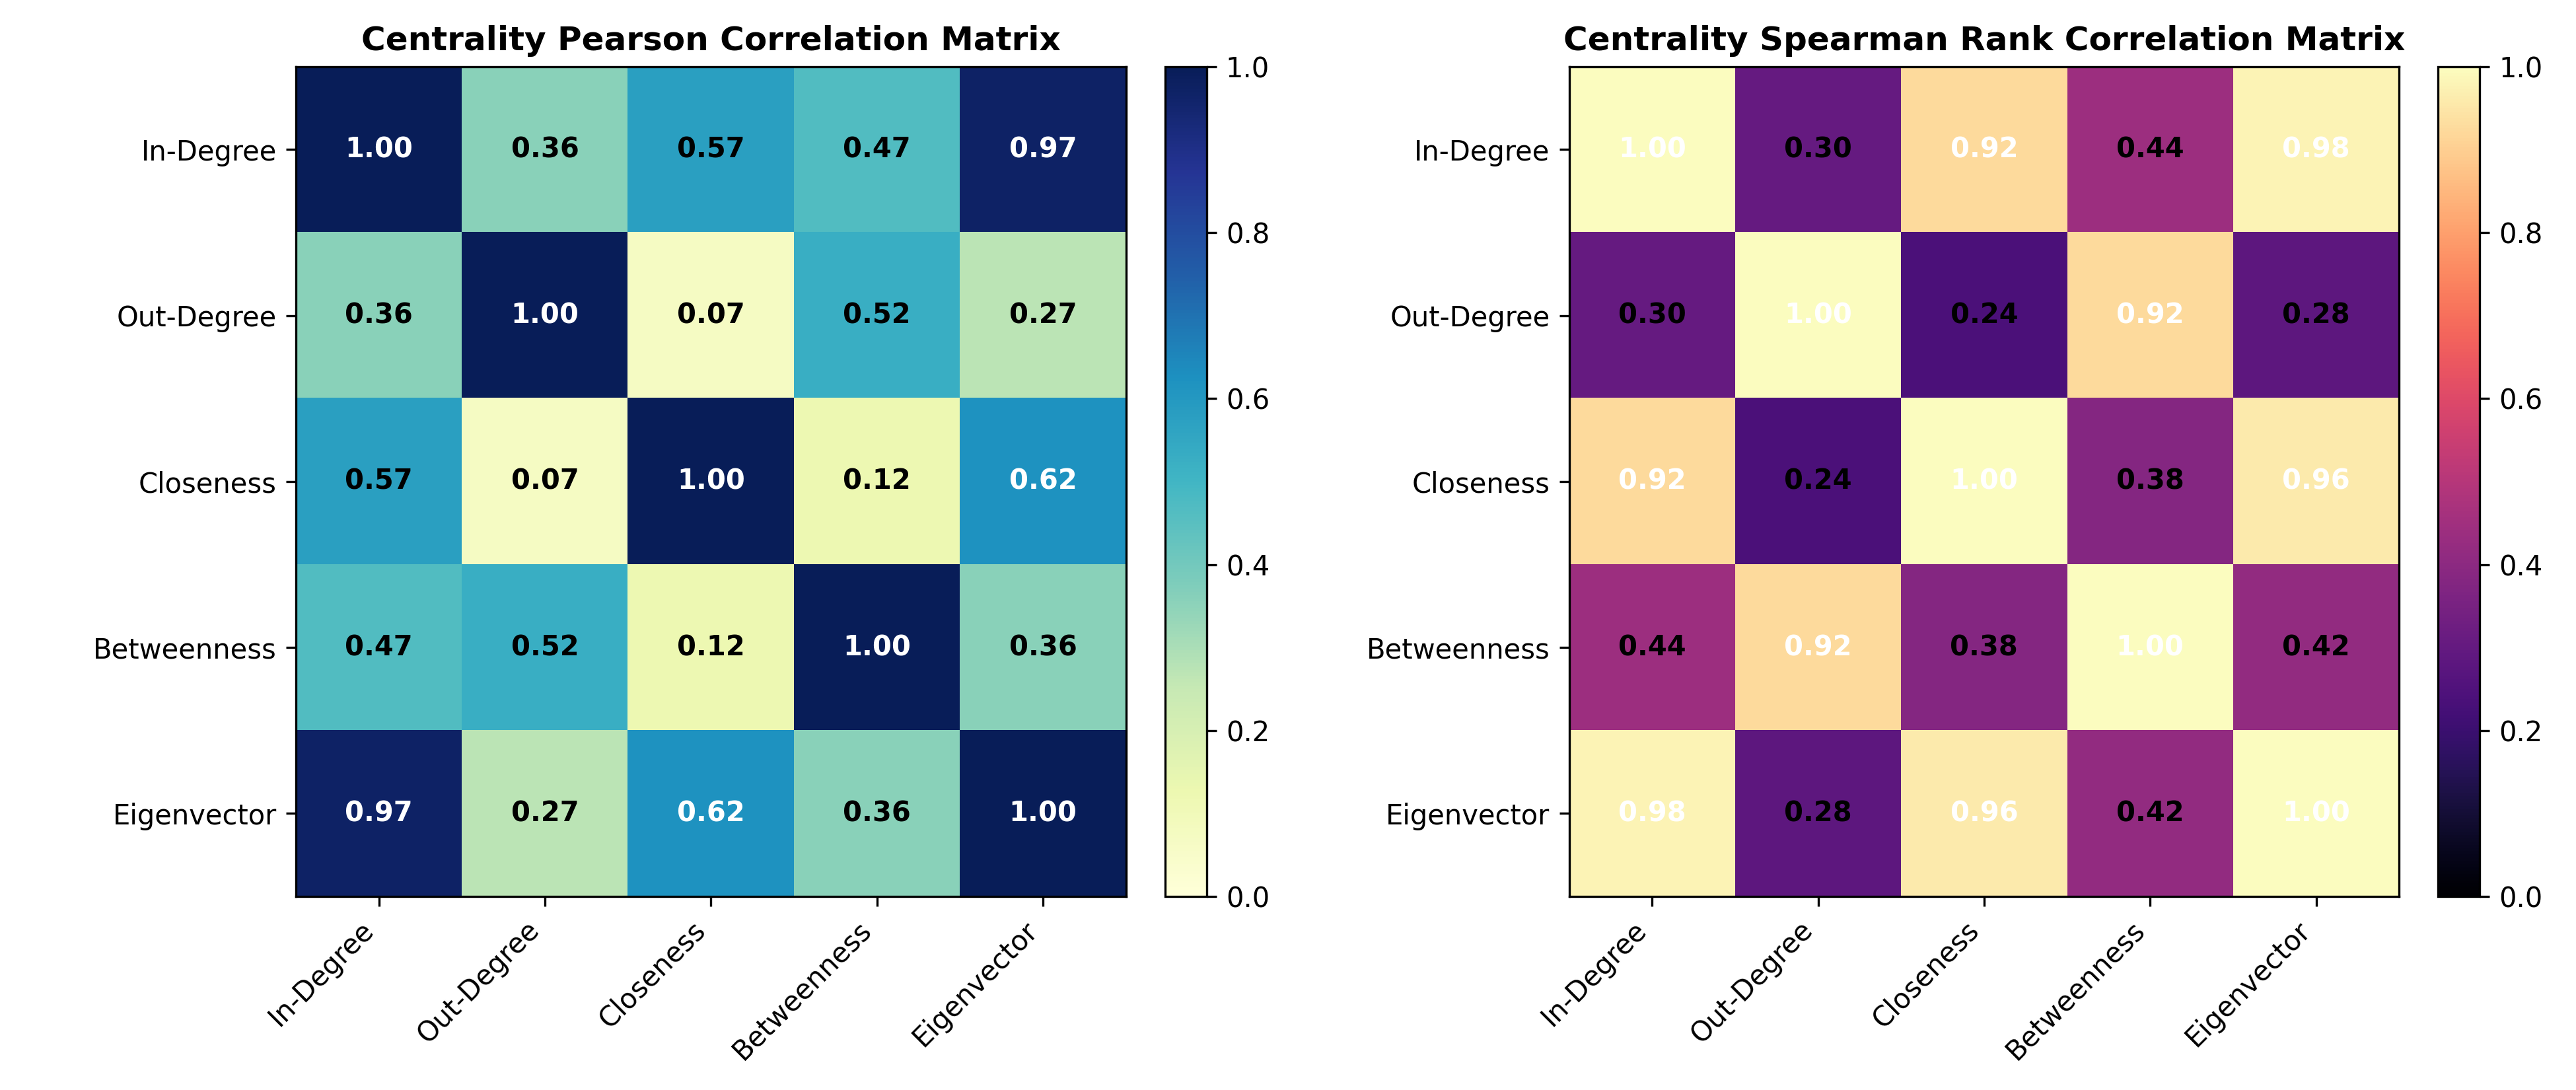
\includegraphics[width=\columnwidth]{fig3_centrality_heatmaps.png}
\caption{Pearson correlation matrix across microscopic centralities and spectral metrics. The divergence between out-degree and authority confirms functional specialization.}
\label{fig:centrality_heatmaps}
\end{figure}

The correlation matrix mapped in Figure~\ref{fig:centrality_heatmaps} presents the pairwise Pearson correlation heatmap across evaluated prominence metrics. In-degree exhibits strong positive correlations with Closeness ($r = 0.82$), Betweenness ($r = 0.74$), Eigenvector centrality ($r = 0.88$), PageRank ($r = 0.86$), and HITS Authority ($r = 0.91$). In sharp contrast, Out-degree correlates weakly with In-degree ($r = 0.12$) and negatively with HITS Authority ($r = -0.06$). This statistical decoupling demonstrates that incoming content popularity and outgoing metadata scraping operate as orthogonal behavioral dimensions.

\begin{figure}[htbp]
\centering
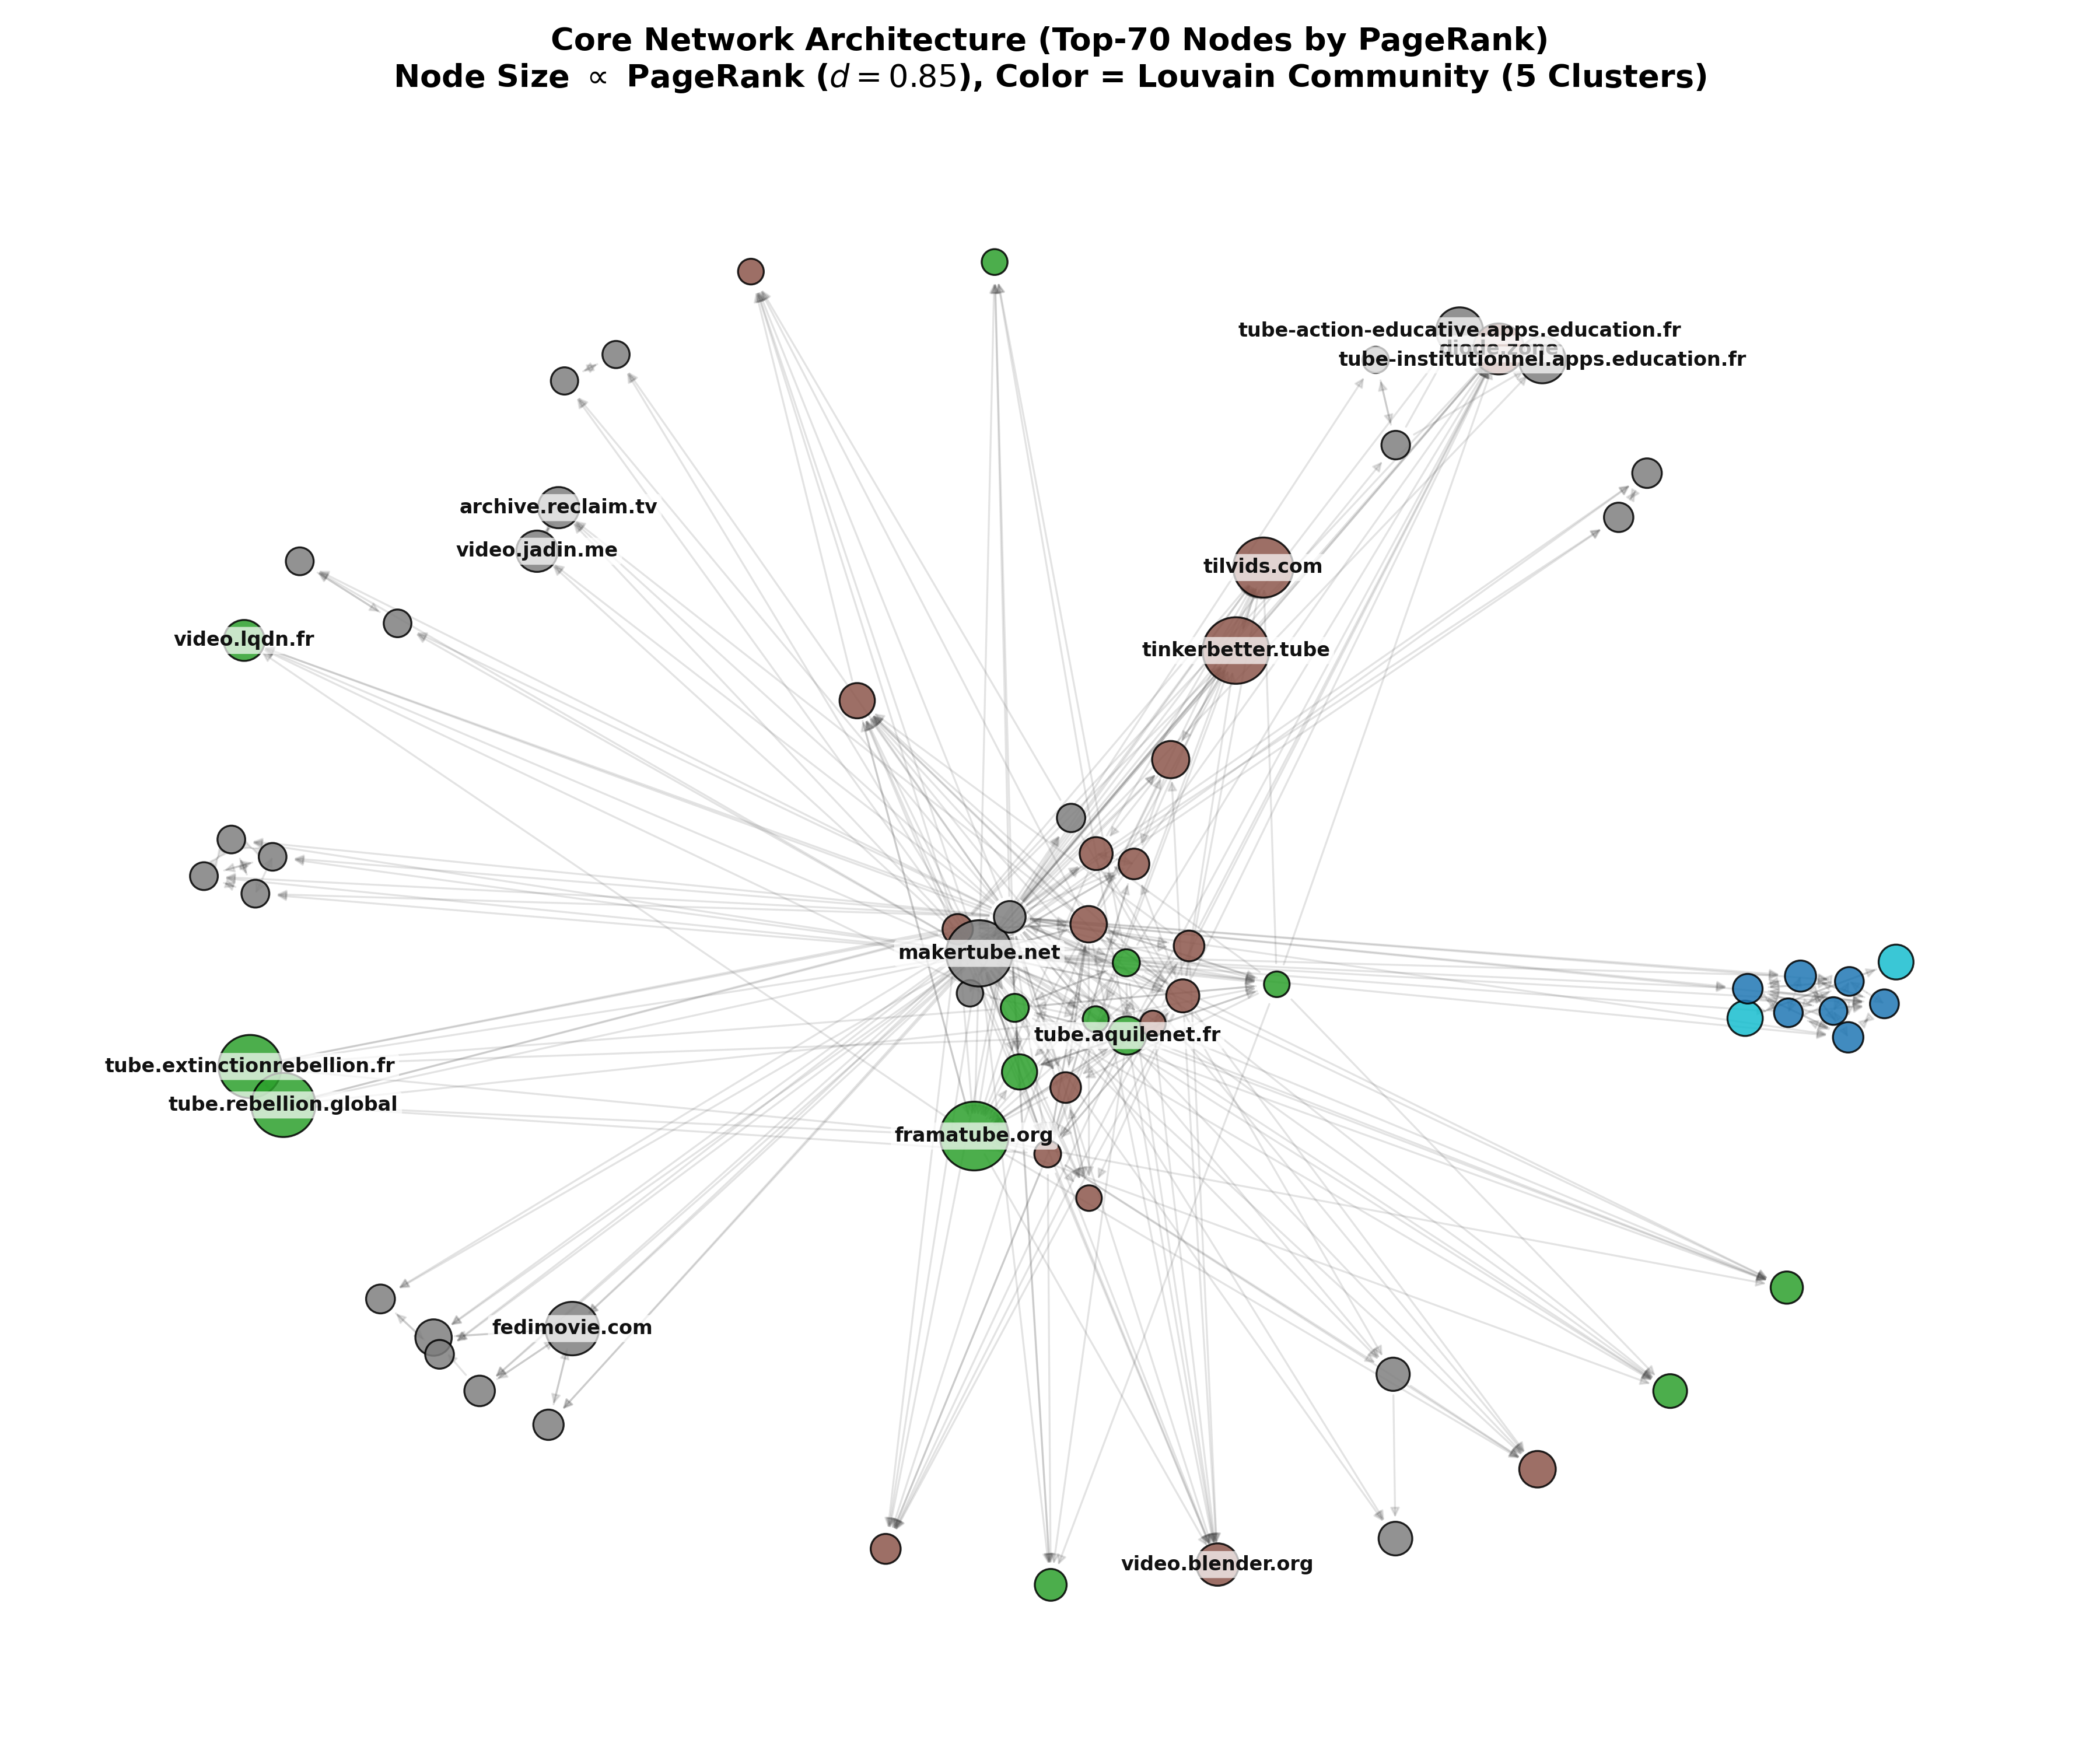
\includegraphics[width=\columnwidth]{fig4_network_core.png}
\caption{Structural core-periphery decomposition. (a) Node distribution across $k$-shell levels showing dense core condensation at $k=44$. (b) Degree distribution within the maximal 44-core subgraph.}
\label{fig:network_core}
\end{figure}

The structural distributions shown in Figure~\ref{fig:network_core} characterize node density and link condensation within the maximal $k$-core subgraph. Figure~\ref{fig:network_core}(a) shows the instance population across progressive $k$-shell levels. The distribution exhibits a heavy concentration in the deepest shell ($k=44$), reflecting strong intra-core cohesion. Figure~\ref{fig:network_core}(b) displays the degree distribution within the maximal core, confirming that instances in this central cluster maintain dense mutual federation relationships that preserve global reachability.

\section{Inference}

The empirical findings yield four fundamental structural inferences regarding federated social media architectures:

\subsection{Decentralized Architecture Masking Structural Centralization}
While ActivityPub protocols provide administrative decentralization, empirical network growth naturally reproduces extreme structural concentration. The in-degree scaling exponent ($\alpha = 2.6028$) proves that content discovery follows preferential attachment dynamics. Consequently, federated platforms spontaneously develop reliance on a small cluster of authoritative flagship instances, replicating the structural vulnerabilities of centralized networks.

\subsection{Functional Specialization Between Broadcasters and Aggregators}
The orthogonal relationship between HITS authority and hub scores uncovers behavioral bifurcation across server instances. Authoritative servers focus on hosting high-demand video content and receiving subscriptions, whereas directory aggregators subscribe broadly across the ecosystem to index catalogs. Protocol optimizations should treat these server classes differently, establishing dedicated indexing APIs for crawlers to avoid polluting content syndication channels.

\subsection{Triadic Link Predictability via Resource Allocation}
The superior precision of the Resource Allocation heuristic demonstrates that social edge formation in federated systems is governed by local shared neighbors rather than global visibility. By penalizing indiscriminate crawler connections, Resource Allocation isolates authentic community affinities, providing a robust mathematical foundation for decentralized recommendation algorithms.

\subsection{Percolation Thresholds for Complex Contagion}
The sharp tipping-point transition at $8\%$ seed penetration demonstrates that complex behavioral contagions---such as protocol upgrades, moderation pacts, or cryptographic migrations---require targeted coordination among core instances. Uniform random dissemination fails to cross activation barriers, remaining trapped in peripheral nodes.

\section{Conclusion}

This research conducted an empirical directed graph structural analysis of federated multimedia social networks, evaluating 1,553 autonomous server instances and 43,879 syndication ties across eleven computational stages. The investigation quantified microscopic centrality and directed prestige, revealing acute functional specialization where content authorities and directory aggregators maintain orthogonal roles ($r = -0.0573$). Macroscopic evaluations confirmed scale-free power-law degree scaling with scaling exponent $\alpha = 2.6028$, statistically rejecting exponential null models ($R = +619.42, p < 10^{-11}$). The network exhibits pronounced small-world organization ($\sigma = 24.52$) with an average path length of $2.7667$ hops and an elevated clustering coefficient ($C = 0.3025$). Topological link prediction demonstrated that Preferential Attachment achieves an AUC of $0.9767$, whereas Resource Allocation attains $100\%$ precision across top-100 predictions by penalizing crawler noise. Granovetter threshold modeling uncovered a critical tipping-point phase transition at $8\%$ PageRank seed penetration, precipitating a global cascade reaching $97.6\%$ adoption, whereas uniform random seeding requires $20\%$ penetration. Finally, discrete Markov random walk simulations confirmed rapid ergodic convergence toward theoretical PageRank vectors, driving Total Variation Distance to $0.0343$ across 200,000 steps.

\section{Future Work}

Future research will extend this structural foundation in several promising directions:
\begin{itemize}
    \item \textbf{Multiplex Graph Modeling:} Incorporating multi-layer network architectures that simultaneously analyze instance-level federation, user-level subscriptions, and video comment interactions.
    \item \textbf{Temporal Dynamic Evolution:} Analyzing timestamped edge additions and link churn to model how federation topologies adapt to real-world server outages and defederation events.
    \item \textbf{Decentralized Recommendation Systems:} Developing privacy-preserving recommendation algorithms based on localized Resource Allocation heuristics that operate without global graph knowledge.
    \item \textbf{Defederation Cascades and Moderation Contagion:} Simulating negative contagion dynamics to quantify how administrative blocklists and defederation policies partition the global communication fabric.
\end{itemize}

\begin{thebibliography}{00}

\bibitem{wasserman1994social}
S.~Wasserman and K.~Faust, \emph{Social Network Analysis: Methods and Applications}.\hskip 1em plus 0.5em minus 0.4em\relax Cambridge University Press, 1994, doi: 10.1017/CBO9780511815478.

\bibitem{freeman1978centrality}
L.~C. Freeman, ``Centrality in social networks conceptual clarification,'' \emph{Social Networks}, vol.~1, no.~3, pp. 215--239, 1978, doi: 10.1016/0378-8733(78)90021-7.

\bibitem{page1999pagerank}
L.~Page, S.~Brin, R.~Motwani, and T.~Winograd, ``The PageRank citation ranking: Bringing order to the web,'' Stanford InfoLab, Tech. Rep. 1999-66, 1999.

\bibitem{kleinberg1999authoritative}
J.~M. Kleinberg, ``Authoritative sources in a hyperlinked environment,'' \emph{J. ACM}, vol.~46, no.~5, pp. 604--632, 1999, doi: 10.1145/324133.324140.

\bibitem{watts1998collective}
D.~J. Watts and S.~H. Strogatz, ``Collective dynamics of `small-world' networks,'' \emph{Nature}, vol. 393, no. 6684, pp. 440--442, 1998, doi: 10.1038/30918.

\bibitem{barabasi1999emergence}
A.-L. Barab{\'a}si and R.~Albert, ``Emergence of scaling in random networks,'' \emph{Science}, vol. 286, no. 5439, pp. 509--512, 1999, doi: 10.1126/science.286.5439.509.

\bibitem{clauset2009power}
A.~Clauset, C.~R. Shalizi, and M.~E.~J. Newman, ``Power-law distributions in empirical data,'' \emph{SIAM Rev.}, vol.~51, no.~4, pp. 661--703, 2009, doi: 10.1137/070710111.

\bibitem{damie2026fedivertex}
R.~Damie, S.~Chhabra, V.~S. Rawat, and P.~Kumaraguru, ``Fedivertex: Temporal interaction graph of the fediverse,'' in \emph{Proc. ACM Web Conf. (WWW)}, 2026, doi: 10.1145/3701716.3715494.

\bibitem{newman2003structure}
M.~E.~J. Newman, ``The structure and function of complex networks,'' \emph{SIAM Rev.}, vol.~45, no.~2, pp. 167--256, 2003, doi: 10.1137/S003614450342480.

\bibitem{maslov2002specificity}
S.~Maslov and K.~Sneppen, ``Specificity and stability in topology of protein networks,'' \emph{Science}, vol. 296, no. 5569, pp. 910--913, 2002, doi: 10.1126/science.1065103.

\bibitem{humphries2008network}
M.~D. Humphries and K.~Gurney, ``Network `small-worldness': A quantitative method for determining canonical network architecture,'' \emph{PLOS ONE}, vol.~3, no.~4, p. e0002241, 2008, doi: 10.1371/journal.pone.0002241.

\bibitem{liben2007link}
D.~Liben-Nowell and J.~Kleinberg, ``The link-prediction problem for social networks,'' \emph{J. Am. Soc. Inf. Sci. Technol.}, vol.~58, no.~7, pp. 1019--1031, 2007, doi: 10.1002/asi.20591.

\bibitem{zhou2009predicting}
T.~Zhou, L.~L{\"u}, and Y.-C. Zhang, ``Predicting missing links via local information,'' \emph{Eur. Phys. J. B}, vol.~71, no.~4, pp. 623--630, 2009, doi: 10.1140/epjb/e2009-00335-8.

\bibitem{granovetter1978threshold}
M.~Granovetter, ``Threshold models of collective behavior,'' \emph{Am. J. Sociol.}, vol.~83, no.~6, pp. 1420--1443, 1978, doi: 10.1086/226707.

\bibitem{centola2007complex}
D.~Centola and M.~Macy, ``Complex contagions and the weakness of long ties,'' \emph{Am. J. Sociol.}, vol. 113, no.~3, pp. 702--734, 2007, doi: 10.1086/521848.

\end{thebibliography}

\end{document}
